\documentclass{article}
\usepackage{amsmath}
\usepackage[parfill]{parskip}
\usepackage{adjustbox}
\usepackage{listings}
\usepackage{graphicx}
\usepackage{color}
\usepackage{hyperref}
\usepackage{tikz}
\def\checkmark{\tikz\fill[scale=0.4](0,.35) -- (.25,0) -- (1,.7) -- (.25,.15) -- cycle;}
\hypersetup{
    colorlinks,
    citecolor=black,
    filecolor=black,
    linkcolor=black,
    urlcolor=black
}
\graphicspath{ {img/} }
\newcommand{\Mod}[1]{\text{ mod }#1}

\lstset{basicstyle=\ttfamily,
  mathescape=true,
  escapeinside=||}

\begin{document}
\title{COMP8411 - Cryptography and Network Security}
\author{Christopher Williamson}
\maketitle
\tableofcontents
\newpage
\section{Introduction}
Cryptography is `the art of keeping messages secure' by scrambling messages so that they can't be understood by unauthorised people.
\begin{itemize}
	\item Plaintext: a message in its original form
	\item Ciphertext: a message in encrypted form
	\item Encryption: code a message to hide its meaning
	\item Decryption: convert an encrypted message back to its original form
	\item Cryptanalysis: attempts to discover plaintext or key
\end{itemize}

\section{The XOR Operator}
\begin{enumerate}
	\item You can apply XOR in any order: $a \oplus b = b \oplus a$, no matter what values $a$ and $b$ are.
	\item Any bit XOR itself is 0: $a \oplus a = 0$.
	\item Any bit XOR 0 is that bit again e.g. if $a$ is 0 then $0 \oplus 0 = 0$, if $a$ is 1 then $1 \oplus 0 = 1$.
\end{enumerate}
The following rules imply that $a \oplus b \oplus a = b$. We'll use this property when using XOR for encryption. The first XOR with $a$ ($a \oplus b$) is the encryption and the second one is the decryption.

\subsection{One-time pads}
This is an encryption scheme that involves a sequence (the `pad') of random bits that is used as the encryption/decryption key. If the bits are truly random and the pad is only used once, the attacker learns nothing about the plaintext when they see the ciphertext. This property is called \textit{perfect security}.

\subsubsection{Reusing the `one-time' Pad}
Suppose an attacker gets two ciphertexts that have been encrypted with the same key. The attacker can then XOR the two ciphertexts, which is also the XOR of the plaintexts.
\begin{center}
	\begin{tabular}{lcll}
	$c1 \oplus c2$ & $=$ & $(p1 \oplus k) \oplus (p2 \oplus k)$ & (definition) \\
	& $=$ & $p1 \oplus k \oplus p2 \oplus k$ & (reorder terms) \\
	& $=$ & $p1 \oplus p2 \oplus k \oplus k$ & ($a \oplus b = b \oplus a$) \\
	& $=$ & $p1 \oplus p2 \oplus 0$ & ($x \oplus x = 0$) \\
	& $=$ & $p1 \oplus p2$ & ($x \oplus 0 = x$) \\
	\end{tabular}
\end{center}
To extract either $p1$ or $p2$, you'd need to know the other plaintext. The problem is that even the result of the XOR operation on two plaintexts contains quite a bit of information about the plaintexts themselves.

\subsubsection{Remaining Problems}
One-time pads are rarely used due to the fact that the key is at least as large as all of the information you'd like to transmit. You also need to ensure that the keys are exchanged securely ahead of time with all of the people you want to communicate with.

Since the keys have to consist of truly random data for it's security property to hold, key generation is fairly difficult and time-consuming without specialised hardware.

\section{Block Ciphers}
A block cipher is an algorithm that allows us to encrypt blocks of a fixed length. It provides an encryption function $E$ that turns plaintext blocks $P$ into ciphertext blocks $C$, using a secret key $k$:
\begin{center}
	$C = E(k, P)$
\end{center}
Once we've encrypted the plaintext blocks into ciphertext blocks, they later have to be decrypted to recover the plaintext. This is done using a decryption function $D$, which takes the ciphertext block $C$ and the key $k$ and returns the original plaintext block $P$.
\begin{center}
	$P = D(k, C)$
\end{center}
Block ciphers are an example of a symmetric-key encryption scheme, also known as a secret-key encryption scheme. This means that the same secret key is used for both encryption and decryption.

A block cipher is a \textit{keyed permutation}. It's a permutation because it maps every possible block to some other block and it's also a \textit{keyed} permutation because the key determines exactly which blocks map to which. This results in a system where knowing a bunch of (input, output) pairs for a given key shouldn't give you any information about any other pairs under that key.

Below are some design criteria for block ciphers:
\begin{itemize}
	\item Completeness - Each bit of the output should depend on every bit of the input and every bit of the key.
	\item Avalanche effect - Changing one bit in the input should change many bits in the output. Also, changing one key bit should result in the change of many bits in the output.
	\item Statistical independence - Input and output should appear to be statistically independent.
\end{itemize}

\subsection{Feistel Block Cipher}
The operation overview for the Feistel block cipher is as follows:
\begin{enumerate}
	\item Initial permutation of bits
	\item Split in half (left \& right)
	\item 16 rounds of identical operations, but each round uses a different sub key
	\item Inverse initial permutation
\end{enumerate}
\begin{center}
	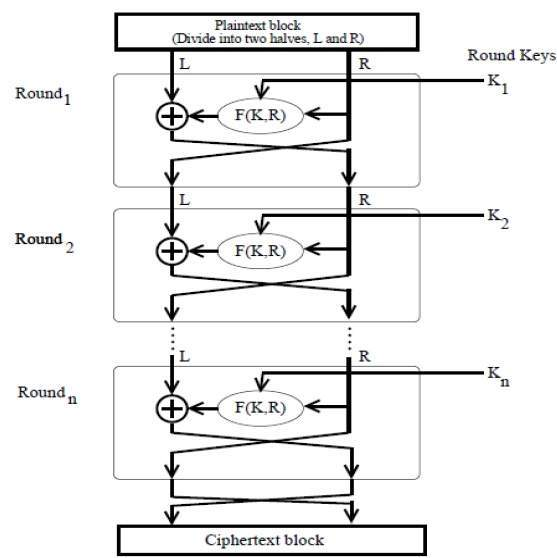
\includegraphics[scale=0.6]{feistel_structure.jpg}
\end{center}
The round function $f$ typically uses permutations, substitutions and modular arithmetic. It take an $n$-bit block and returns an $n$-bit block. A larger block size, $n$, means greater security but makes encryption/decryption slower. It is typically 128 or 256 bits. The key size follows the same principles, 128-bits is the norm. Finally, the number of rounds, $r$ is usually over 10.

\subsection{Data Encryption Standard (DES)}
DES was first published in 1977 as a US Federal standard and is a de facto international standard for banking security. it's a feistel block cipher whose block length is 64 bits and key is 56 bits. The sub-keys, $k1, k2...k16$ are each 48-bits and are generated from the main key. The decryption algorithm is exactly the same as the encryption algorithm except that the keys for each round must be used in reverse order.

\subsubsection{DES Round Function}
\begin{enumerate}
	\item Expansion permutation - Right half is expanded (and permuted) to 48 bits. This diffuses the relationship of input bits to output bits.
	\item Use of round key - All 48 bits of the round key are XOR-ed with out 48 bits from step 1.
	\item Splitting - The result is split into eight lots of six bits each.
	\item S-box (substitution) - Each six bit block is used as an index to an S-box to produce a 4 bit result (so we'll get eight 4 bit blocks).
	\item P-box (permutation) - The 32 bits of output from step 4 are permuted which gives us the output of our round function.
\end{enumerate}
For the S-box step there are 8 different S-boxes, one for each block. Each of these is a table of four rows and 16 columns. The 6 input bits specify which row and column to use for the index of the table. Bits 1 and 6 select the row, bits 2-5 select the column. The decimal value in that cell is then converted to a 4-bit result.

\subsubsection{Triple DES}
Triple DES involves the use of two or three DES keys.

EDE2 is triple DES using two keys, therefore the key length is 112 bits:
\begin{center}
	$C=E_{K1}(D_{K2}(E_{K1}(M)))$
\end{center}
EDE3 is triple DES using three keys, therefore the key length is 168 bits:
\begin{center}
	$C=E_{K3}(D_{K2}(E_{K1}(M)))$
\end{center}

\subsection{Advanced Encryption Standard (AES)}
This is the most common block cipher in current use. It was selected through a public, peer-reviewed competition.
\begin{itemize}
	\item Block size: 128 bits (called a state)
	\item Key sizes: 128, 192 or 256 bits
\end{itemize}
AES consists of several independent steps. At a high level, AES is a substitution-permutation network involving $r$ rounds.
\begin{center}
	\begin{tabular}{|c|c|}
		\hline
		Key length & Rounds \\ \hline
		128 & 10 \\
		192 & 12 \\
		256 & 14 \\
		\hline
	\end{tabular}
\end{center}
A single round transformation consists of the following steps:
\begin{itemize}
	\item Byte substitution.
	\item Shift rows.
	\item Mix columns.
	\item Round key addition.
\end{itemize}
Note that in practice, the round key addition step if done before the rounds start, and in the last round, the mix columns step is not performed.

Shift rows and mix columns provide diffusion, that is, changing one bit of the input changes many bits of the output thus achieving the avalanche effect.

Byte substitution provides statistical independence as the look-up tables are very non-linear thus good at destroying patterns.

Round key addition provides completeness as the whole key is used to derive the round keys and the whole input is used for encryption.

\subsection{DES vs AES}
\begin{center}
	\begin{tabular}{p{6cm}p{6cm}}
		\multicolumn{1}{c}{\textbf{DES}} & \multicolumn{1}{c}{\textbf{\textbf{AES}}} \\
		Substitution-permutation, iterated cipher, feistel structure & Substitution-permutation, iterated cipher \\
		64-bit block size, 56-bit key size & 128-bit block size, 128-bit (192, 256) key sizes \\
		8 different S-boxes & 1 S-box \\
		Design optimised for hardware implementations & design optimised for byte-orientated implementations. \\
		Closed (secret) design process & Open design and evaluation process \\
	\end{tabular}
\end{center}

\subsection{Other Symmetrical Cryptosystems}
\begin{center}
	\begin{tabular}{|l|l|l|}
	\hline
	Algorithms & Mode (block length in bits) & Key length (bits) \\ \hline
	DES & Block cipher (64) & 56 \\ \hline
	Triple DES & Block cipher (64) & 168 $(=3*56)$ (112 effective) \\ \hline
	Rijndael & Block cipher (128, 192 or 256) & 128, 192 or 256 \\ \hline
	Blowfish & Block cipher (64) & variable up to 448 \\ \hline
	IDEA & Block cipher (64) & 128 \\ \hline
	RC5 & Block cipher (32, 64, 128) & Variable up to 2040 \\
	\hline
	\end{tabular}
\end{center}

\subsection{Modes of Operation - Encrypting Large Messages}
If a message is longer than its block size, the block cipher can be used in a variety of ways to encrypt the plaintext. There are a number of modes of operations, below are three of them:
\begin{itemize}
	\item ECB - Electronic Code Book mode
	\item CBC - Cipher Block Chaining mode
	\item CTR - Counter mode
\end{itemize}
These modes of operation have been standardised internationally and are applicable to any block ciphers.

\subsubsection{ECB Mode}
In this mode, each block is encrypted independently using the same key. The last block should be padded if necessary. Usually the last byte indicates the number of padding bytes added; this allows the receiver to remove the padding. The blocks are then encrypted independently of each other. Reordering the ciphertext blocks will result in correspondingly reordered plaintext blocks.

\subsubsection{CBC Mode}
In this mode the plaintext is divided into blocks and the last block is padded if necessary. Ciphertext block $C_{j}$ depends on plaintext block $M_{j}$ \textbf{and all preceding plaintext blocks}:
\begin{center}
	$C_{n} = E_{k}(M_{n} \oplus C_{n-1})$ \\
	$C_{0} = IV$ (Initialisation vector)
\end{center}

\subsubsection{CTR Mode}
A counter, equal to the plaintext block size is used. The counter value must be different for each plaintext block. Typically the counter is initialised to some value, and then incremented by 1 for each subsequent block (modulo $2^{n}$, where $n$ is the block length).

Each block can be decrypted independently of the other, therefore it can be run in parallel and there is also no error propagation.

\subsection{Block Ciphers vs Stream Ciphers}
While block ciphers encrypt blocks of characters, stream ciphers encrypt individual characters or bit streams.

Stream ciphers:
\begin{itemize}
	\item Are usually faster than block ciphers in hardware; mostly used for continuous communications and/or real-time applications.
	\item Requires less memory space, so cheaper for resource restrained devices such as embedded sensors.
	\item Have limited or no error propagation, so advantageous when transmission errors are probable.
	\item Can be build out of block ciphers, e.g. by using CTR modes.
\end{itemize}

\section{Public Key Cryptography}
Up to this point, all cryptographic schemes are based on shared secret-keys (symmetric cryptography). One major problem with symmetric cryptography is that a separate key is needed for each pair of users. Therefore, an $n$-user system requires $n*(n-1)/2$ keys - the $n^{2}$ problem. Generating and distributing these keys is also a challenging problem and maintaining security for already distributed keys is challenging. Finally, as two parties share the same key, non repudiation can not be achieved. It was in 1976 that Diffie and Hellman first presented the concept of public key cryptography.
\begin{itemize}
	\item Based on mathematically hard problems rather than substitution/transposition.
	\item A pair of keys is used, public and private. Pair are related mathematically.
	\item Encryption generated by one key can only be decrypted by the other key in that pair.
	\item Examples: RSA, DSS, DH (Diffie Hellman).
\end{itemize}

\subsection{Achieving Confidentiality}
Our scenario is that Alice wants to send a message to Bob and ensure that is has confidentiality protection.
\begin{enumerate}
	\item Alice encrypts the message with Bob's \textbf{public} key
	\item Bob decrypts Alice's message with his \textbf{private} key
\end{enumerate}
This method ensures that only Bob can decrypt the ciphertext (as he is the only one in possession of his private key). Usually this is only applied to short messages, e.g. for secure transmission of symmetrical keys.

\subsection{Achieving Authenticity}
Our scenario here is that Alice wants to send a message to Bob and Bob wants to be assured that the message has come from Alice.
\begin{enumerate}
	\item Alice signs the hash value of the plaintext with her \textbf{private} key
	\item Bob verifies the hash value using Alice's \textbf{public} key
\end{enumerate}
Usually the signature is signed in the hash value of the plaintext, and a timestamp should also be included.

\subsection{Modulo Operator}
\begin{center}
	$a \equiv b \Mod n$
\end{center}
Means that there exists an integer number $k$ such that $a$ can be represented as:
\begin{center}
	$a \equiv k \cdot n + b$
\end{center}
Given integers, $a$, $b$, and $n \neq 0$. $a$ is congruent to $b \Mod n$ iff $a-b \equiv k\cdot n$ for some integer $k$.

Examples:
\begin{itemize}
	\item $9 \Mod 5 = 4$
	\item $20 \Mod 9 = 2$
	\item $17 = 2 \Mod 5$ since $17-2 = 3 \cdot 5$
\end{itemize}
Below are some properties of modular arithmetic:
\begin{itemize}
	\item $a \equiv a \Mod n$
	\item $a \equiv b \Mod n \leftrightarrow b \equiv a \Mod n$
	\item $a \equiv b \Mod n \text{ \& } b \equiv c \Mod n \rightarrow a \equiv c \Mod n$
	\item $(a + b) \Mod n = ((a \Mod n) + (b \Mod n)) \Mod n$
	\item $(a \cdot b) \Mod n = ((a \Mod n) \cdot (b \Mod n)) \Mod n$
	\item $a \cdot (b + c) \Mod n = (a \cdot b + a \cdot c) \Mod n$
	\item $a \cdot x \Mod n = 1$ where $x$ is an integer and called the multiplicative inverse of $a$
\end{itemize}
Below is some code that finds the multiplicative inverse of $a$ under $n$:
\begin{lstlisting}
def multiplicative_inverse(a, n):
  x = 1

  while x < n:
    if (a*x) % n == 1:
      return x
    else:
      x += 1
\end{lstlisting}
$a$ and $b$ are said to be relatively prime if only 1 can divide each of them e.g. 8 and 15.
\subsection{RSA Algorithm}
The RSA algorithm was invented by Ron \textbf{R}ivest, Ali \textbf{S}hamir and Leonard \textbf{A}dleman. It has withstood years of cryptanalysis and remains by far the most popular and well trusted scheme.

The algorithm consists of two numbers, the modulus, $n$, and the public exponent, $e$. The modulus is a product of two very large prime numbers (100 to 400 digits), represented by the letters $p$ and $q$. They need to be kept secret.

It is a block cipher in which the plaintext and ciphertext are integers between 0 and $n-1$ for some $n$.

\subsubsection{Key Generation}
\begin{enumerate}
	\item Select two large primes, $p$ and $q$
	\item Calculate $n = p \cdot q$ and $\phi(n) = (p-1) \cdot (q-1)$
	\item Select an integer, $e$ which is relatively prime to $\phi(n)$ and $1 < e < \phi(n)$
	\item Calculate a value $d$ such that $d = e^{-1} \Mod \phi(n)$ or $(d \cdot e) \Mod \phi(n) = 1$
	\item Public key = ${e, n}$
	\item Private key = ${d, n}$
\end{enumerate}
You can see that $e$ is \textbf{publicly} chosen and $d$ is \textbf{private} and calculated.

\subsubsection{Encryption}
For the plaintext, we represent it as an integer $M$ in the range $0 < M < n$. The ciphertext is then:
\begin{center}
	$C = M^{e} \Mod n$
\end{center}

\subsubsection{Decryption}
To get the plaintext from the ciphertext we use the private key, ${d, n}$:
\begin{center}
	$M = C^{d} \Mod n$
\end{center}

\subsubsection{Worked Example}
\begin{enumerate}
	\item Select $p=7$ and $q=17$
	\item Calculate $n = p \cdot q = 119$
	\item Calculate $\phi(n) = (p-1) \cdot (q-1) = 96$
	\item Select $e = 5$, which is relatively prime and less than $\phi(n)$
	\item Calculate $d=77$ such that $de \Mod \phi(n) = 1$
	\item Let $M = 19$, then $C = 19^{5} \Mod 119 = 66$
\end{enumerate}

PKCS\#1 standard defines the use of the RSA algorithm. It defines the key generation, encryption, decryption, digital signatures, verification, public key format, padding, and several other issues with RSA: \url{https://en.wikipedia.org/wiki/PKCS_1}

The security of RSA relies on the difficulty of finding $d$ given ${e, n}$. $p$ and $q$ should differ in length by only a few digits, and both should be on the order of 100 - 200 digits or even larger.
\begin{itemize}
	\item $n$ with 150 digits could be factored in about 1 year
	\item Factoring $n$ with 200 digits could take about 1000 years
\end{itemize}
\subsection{Hybrid Cryptosystems}
Public key ciphers are much slower than symmetrical key ciphers, 1000 times slower in hardware, and 100 times slower in software, than DES. Symmetric ciphers also have key management problems and can not provide non-repudiation service without the involvement of a trusted third party.

Due to these issues, we usually combine them to get the strengths of both - this leads to the hybrid cryptosystem:
\begin{itemize}
	\item Public cipher for symmetric key establishment/transportation and/or digital signature generation.
	\item Symmetric cipher for bulk encryption.
\end{itemize}
The technique is called digital enveloping. A symmetrical algorithm with a random session key is used to encrypt the message and then a public-key algorithm is used to encrypt the random session key.

\section{Cryptographic Checksums}
Conventional symmetric encryption: $a \rightarrow B: E_{k}[M]$ provides confidentiality, as ONLY $A$ and $B$ share $K$. It also provides a certain degree of origin authentication as it could only come from $A$. It does not provide signature as receiver $B$ could also generate the encryption and sender $A$ could deny sending the message (repudiation of origin).

Public key encryption: $A \rightarrow B: E_{KUb}[M]$ provides confidentiality but not origin authentication as everyone knows $B$s private key.

Digital signing is applied in the following manner:
\begin{center}
  $A \rightarrow B: M \| E_{KR_{a}}[h(M)]$
\end{center}
Which means that we have the plaintext, $M$, with the encrypted hash value of $M$ attached to the end of it. The encryption is done with $A$s private key. This method provides origin authentication and non-repudiation as:
\begin{itemize}
  \item Only $A$ has $KR_{a}$, so signed item must have come from $A$.
  \item Any party can use $KU_{a}$ to verify the item.
  \item Provided $KU_{a}$ is trust-worthy, and the signature is dated.
\end{itemize}
But it does not provide confidentiality.

Some of the cryptographic operations mentioned above could only provide message authentication and integrity protections provided that the message has some structures or is recognisable. We therefore need some redundancy for the receiver to verify the message - this check-value is a \textbf{cryptographic checksum}.

A cryptographic checksum can be used to protect:
\begin{itemize}
  \item Content authentication (origin + integrity)
  \item Non-repudiation
  \item Anti-replay
\end{itemize}

\subsection{Digest Function}
Given a message, $M$, of arbitrary length, a Message Digest function, $H$, produces a fixed-size output, $h$ (called a message digest, checksum, hash value, or fingerprint, of $M$). $h$ should be a function of all the bits of $M$

\subsubsection{Requirements}
A message digest function should take into account the following properties:
\begin{itemize}
  \item \textbf{Compression}: $H$ can be applied to a block of data of any size, but produces a fixed-length output.
  \item \textbf{One-way property}: $H(x)$ is easy to compute for any given $x$. For any given $h$, it is hard to compute $x$ such that $H(x) = h$.
  \item \textbf{Weak collision resistance}: Given $x$, it is hard to find $y \neq x$ such that $H(y) = H(x)$.
  \item \textbf{Strong collision resistance}: It is hard to find two different messages, $x \neq y$, such that $H(y) = H(x)$.
\end{itemize}
If $H$ is strong collision resistant, it is also weak collision resistant.

If the weak collision resistance property is not met signature forgery is likely. Assuming that $A$ has sent a signed message $M$ to $B$, $M \| s$ where $s=R_{KR_{a}}[H(M)]$:
\begin{enumerate}
  \item An attacker intercepts $A$'s signature and message.
  \item The attacker finds another message, $M'$ where $H(M) = H(M')$.
  \item The attacker now has your signature $s$ on the real message.
\end{enumerate}
Repudiation is likely if the strong collision resistance property is not met. Assuming that $A$ is to send a signed message $M$ to $B$:
\begin{enumerate}
  \item $A$ chooses two messages $M$ and $M'$ where $H(M) = H(M')$.
  \item $A$ signs $M$ by generating the signature.
  \item $A$ sends $B$ $M \| s$.
  \item Later $A$ repudiates this signature, saying that it was really a signature on the message $M'$.
\end{enumerate}

\subsection{Construction Methods}
Cryptographic checksum construction methods include message authentication code (MAC), hash functions and HMAC, among others. Below we take a deeper look into some of these construction methods.

\subsubsection{Extension Method}
In this method, each MD function processes a block of $M$, the output is the input for the next block. The output of the final block is the digest of the entire message.

\subsubsection{Message Authentication Code (MAC)}
This is a public function with a shared secret key that produces a fixed-length output i.e. $\text{MAC} = f_{k}(M)$.

It is block cipher based which means that it is slow and produces a short digest length. As before, the output of one block is the input to the next block. At the end we just take the last output value as our digest.

If only $A$ and $B$ know the secret key $K$, and if $\text{MAC} = \text{MAC}'$ (MAC' is the receivers digest), then the receiver can be assured that:
\begin{itemize}
  \item The message has not been altered.
  \item The message is from the alleged sender.
  \item The message is of the proper sequence if the message includes a sequence number.
  \item The message is fresh, if the message includes a timestamp.
\end{itemize}

\subsubsection{Hash Functions}
Below is a table of commonly used hash functions:
\begin{center}
  \begin{tabular}{|l|l|l|l|l|}
    \hline
    & SHA-1 & SHA-256 & SHA-384 & SHA-512 \\ \hline
    Hash value size & 160 & 256 & 384 & 512 \\ \hline
    Block size & 512 & 512 & 1024 & 1024 \\ \hline
    Word size & 32 & 32 & 64 & 64 \\ \hline
    Security & 80 & 128 & 192 & 256 \\
    \hline
  \end{tabular}
\end{center}
Security refers to the fact that a birthday attack on a message digest of size $n$ produces a collision with a work-factor of approximately $2^{n/2}$.

\subsubsection{HMAC}
HMAC constructs MAC by applying a message and key to a cryptographic hash function in a nested manner i.e.
\begin{center}
  $\text{HMAC}(K, M) = H[(K \oplus \text{opad}) \| H[(K \oplus \text{ipad}) \| M)]]$
\end{center}
Where:
\begin{itemize}
  \item \textbf{H}: hash function such as SHA-1
  \item \textbf{ipad}: a string by repeating the byte 0x36 (00110110) as often as necessary.
  \item \textbf{opad}: a string by repeating the byte 0x5c (01011100) as often as necessary.
  \item \textbf{K}: 512-bits secret key
\end{itemize}

\section{Digital Signature Algorithms}
A digital signature associates a mark unique to an individual with a body of text. It should be:
\begin{itemize}
  \item Message-dependent: unreusable \& ensures integrity
  \item Signer-dependent: unforgable \& ensures authenticity
  \item Verifiable: others should be able to verify that the signature is indeed from the originator.
\end{itemize}
A digital signature scheme uses public-key cryptography, typically RSA or DSA.

The main idea is that only $A$ can sign a message because only $A$ has access to their private key. Anyone can verify $A$'s signature because everyone has $A$'s public key. A digital signature scheme consists of a key generation algorithm, a signature generation algorithm and a signature verification algorithm.

\subsection{RSA Signature Generation}
In this scenario, Alice wants to send Bob a signed message so that Bob knows that it is Alice who has sent the message.

Alice has a public and private key: $KU_{a} = \{e, n\}$ and $KR_{a} = \{d, n\}$. Bob also has access to Alice's public key.

Alice generates a signature in the following way:
\begin{center}
  $S = M^{d} \Mod n$
\end{center}
She then attached this to her message and sends to Bob: $A \rightarrow B: M\|S$.

Bob receives the message: $M'\|S$. And works out M:
\begin{center}
  $M = S^{e} \Mod n$
\end{center}
If $M$ matches $M'$, the signature is valid and Bob can be sure that Alice sent the message.

\subsection{RSA for Digital Signature - Problems}
One problem with using RSA for digital signature is that RSA can only handle so much data and we may want to sign a message which is longer than RSA allows. One way to solve this would be to break the message up into smaller chunks but this would add a great deal of complexity and expense.

There is also a security issue:
\begin{itemize}
  \item Let $m$ be the message of which you want to forge a signature.
  \item Choose two messages $x$ and $y$ such that $xy = m \Mod n$.
  \item If you could obtain the signatures of $x$ and $y$ then you can easily forge a signature of $m$ by $S(m) = S(y)S(x) \Mod n$
\end{itemize}
A solution to these problems is to use the `hash-and-sign' paradigm where we sign the hash value of the message. Below is how we write the signature generation process and the signature verification process:
\begin{center}
  $S=E_{KR_{a}}[H(M)]$ \\
  $h=D_{KU_{a}}[S] = D_{KU_{a}}[E_{KU_{a}}[H(M)]]$
\end{center}
The remaining problem is how can we ensure that public keys are trustworthy? This is covered in the Public Key Infrastructure topic.

\subsection{DSA}
Below is an illustration of the workings of the DSA algorithm:
\begin{center}
  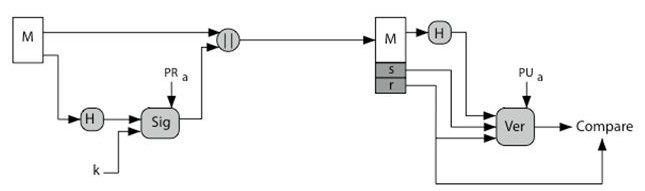
\includegraphics[scale=0.6]{dsa.jpg}
\end{center}
$k$ is a random number generated for this signature (it should be different for every signature generation). $PR_{a}$ is the sender's private key and $PR_{a}$ is the sender's public key.

\subsubsection{Key Generation}
First we generate our global public-key components that can be shared among a group of users:
\begin{itemize}
  \item Choose $p$, a 512-bit to 2048-bit prime number.
  \item Choose $q$, a 160-bit prime number which divides $(p-1)$ ($q$ is a prime divisor of $p-1$).
  \item $g = h^{(p-1)/q} \Mod p$ where $h$ is any integer where $1 < h < (p-1)$ such that $h^{(p-1)/q} \Mod p > 1$.
\end{itemize}
Next, we choose a long-term private key, $x$, which should be a randomly chosen value in the range $0 < x < q$. Now we can compute our long-term public key:
\begin{center}
  $y = g^{x} \Mod p$ \\
  $KU_{a} = \{p, q, g, y\}$
\end{center}

\subsubsection{The Signing Process}
Once we have our public/private key pair, we can move onto the signing stage. First, we choose a random number for $k$. This key must be destroyed after use and must never be reused. We then compute two components:
\begin{itemize}
  \item $r = (g^{k} \Mod p) \Mod q$
  \item $s = [k^{-1}(H(M) + xr)] \Mod q$
  \item $\text{Signature} = (r, s)$
\end{itemize}
We can then send $M \| \text{signature}$ to the receiver.

\subsubsection{Signature Verification}
So now the receiver has got $KU_{a}$ and $\{M', r', s'\}$. We compute:
\begin{itemize}
  \item Message hash $H(M')$
  \item mod $q$ inverse of $s'$: $w = (s')^{-1} \Mod q$
  \item $u_{1} = [H(M')w] \Mod q$
  \item $u_{2} = (r')w \Mod q$
  \item $v = [(g^{u_{1}}y^{u_{2}}) \Mod p] \Mod q$
\end{itemize}
We then test that $v = r'$. If this is true, then the signature is verified.

\subsection{RSA vs DSA}
\begin{tabular}{|p{6cm}|p{6cm}|}
  \hline
  \multicolumn{1}{|c|}{\textbf{RSA}} & \multicolumn{1}{|c|}{\textbf{\textbf{DSA}}} \\ \hline
  Security is based on difficulty of factoring large numbers & Security is based on difficulty of taking discrete logarithms \\ \hline
  Can encrypt and sign & Can only sign messages \\ \hline
  Faster than DSA in signature verification, and about the same in signature generation. & Some signature computation can be computed priori. \\ \hline
  Can recover the message digest from the signature & Cannot recover the message digest from the signature \\ \hline
  & Need to choose a unique secret number $k$ for each message \\
  \hline
\end{tabular}

\section{Public Key Infrastructure}
The major problem with wide-scale application of public-key cryptography is how can we trust that a given public key belongs to the claimed entity? The solution is to have someone or some authority to sign one's public key (a digital certificate). A digital certificate is a statement certifying that this public key belongs to this identity and the owner with this identity possesses the corresponding private key.

\subsection{Two Trust Models}
SPKI (Simple PKI) is a bottom-up approach:
\begin{itemize}
  \item Uses a web-of-trust model.
  \item Public keys are signed/certified by friends or friends' friends.
  \item You are supposed to trust some of the friends.
  \item Used in the PGP solution.
\end{itemize}
X509 PKI is a top-down approach:
\begin{itemize}
  \item Public keys are signed/certified by trusted authorities, Certification Authorities (CAs).
  \item A CA or CA hierarchy digitally sign keys in a top-down manner.
\end{itemize}
Below is a diagram showing the connections between PKI entities:
\begin{center}
  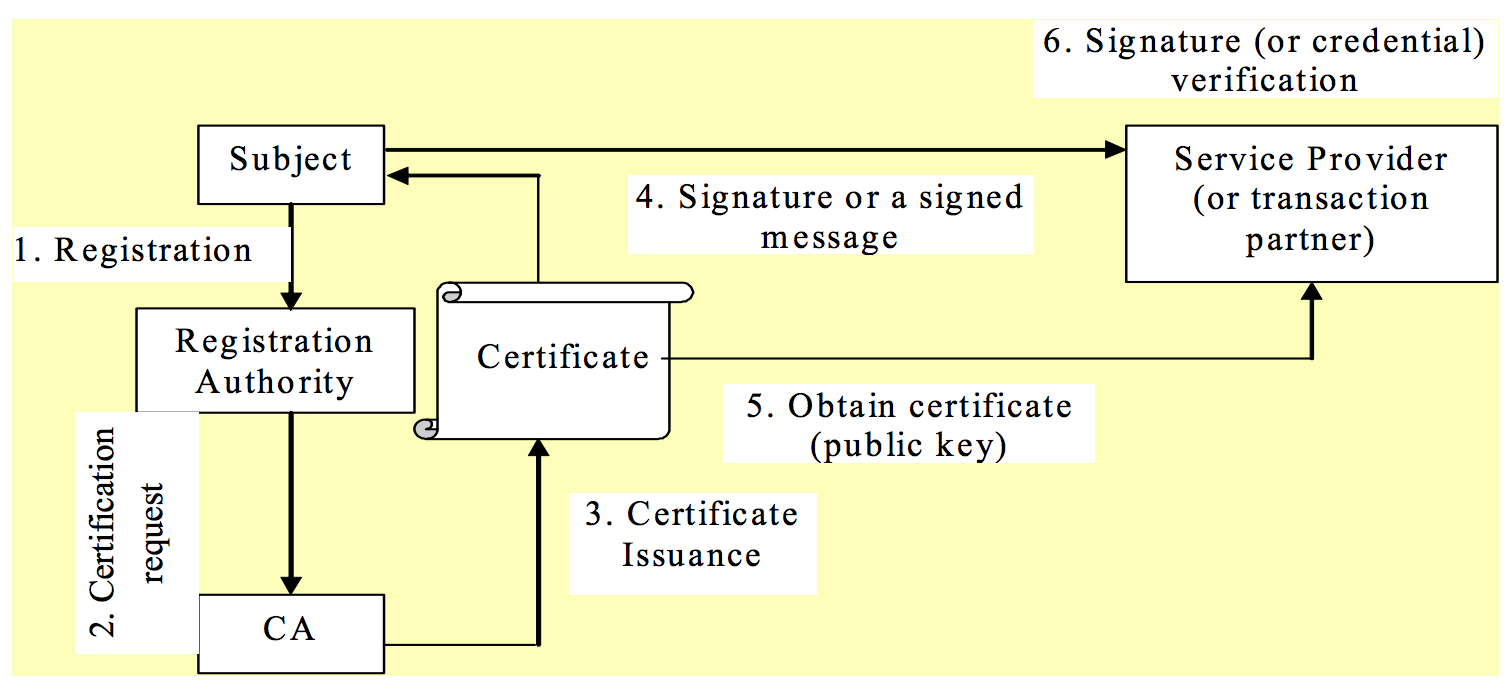
\includegraphics[scale=0.5]{pki.png}
\end{center}

\subsection{Main Functions}
\subsubsection{SystemSetup}
A credential service provider should get the policy, procedures and services ready, including key generation/update, certificates issuance, distribution and revocation, possibly key recovery, and potential interaction with other providers.
\subsubsection{SubjectRegistration}
During this process, a subject makes itself known to a CA.
\subsubsection{KeyGeneration}
A pair of crypto keys are generated either by the subject or by the CA, and the CA will certify the public key of the pair.
\subsubsection{CredentialIssuance}
The CA issues a certificate for a subject's public key.
\subsubsection{CredentialVerification}
This is performed when a credential is used to access a service or to perform a transaction
\subsubsection{CredentialRevocation}
If the private key associated to the public key certified in the certificate is compromised or suspected compromised, then the certificate should be revoked.
\subsubsection{Cross-certification}
Is an operation to allow a pair of CAs to establish a trust relationship through the signing of each other's public keys in a certificate called cross-certification.
\subsubsection{SubjectRegistration}
\textbf{Enrollment:} An applicant, e.g. Alice, may need to provide the following information:
\begin{itemize}
  \item Proof of Alice's identity
  \item Alice's public key
\end{itemize}
\textbf{Authenticates applications:}
\begin{itemize}
  \item Share information with a third-party database
  \item Personal appearance
\end{itemize}
A Data Repository, typically a LDAP directory is where certificates and revocation status are officially stored
\subsection{The X.509 v3 Certificate Format}
The image below is the structure of this type of certificate format:
\begin{center}
  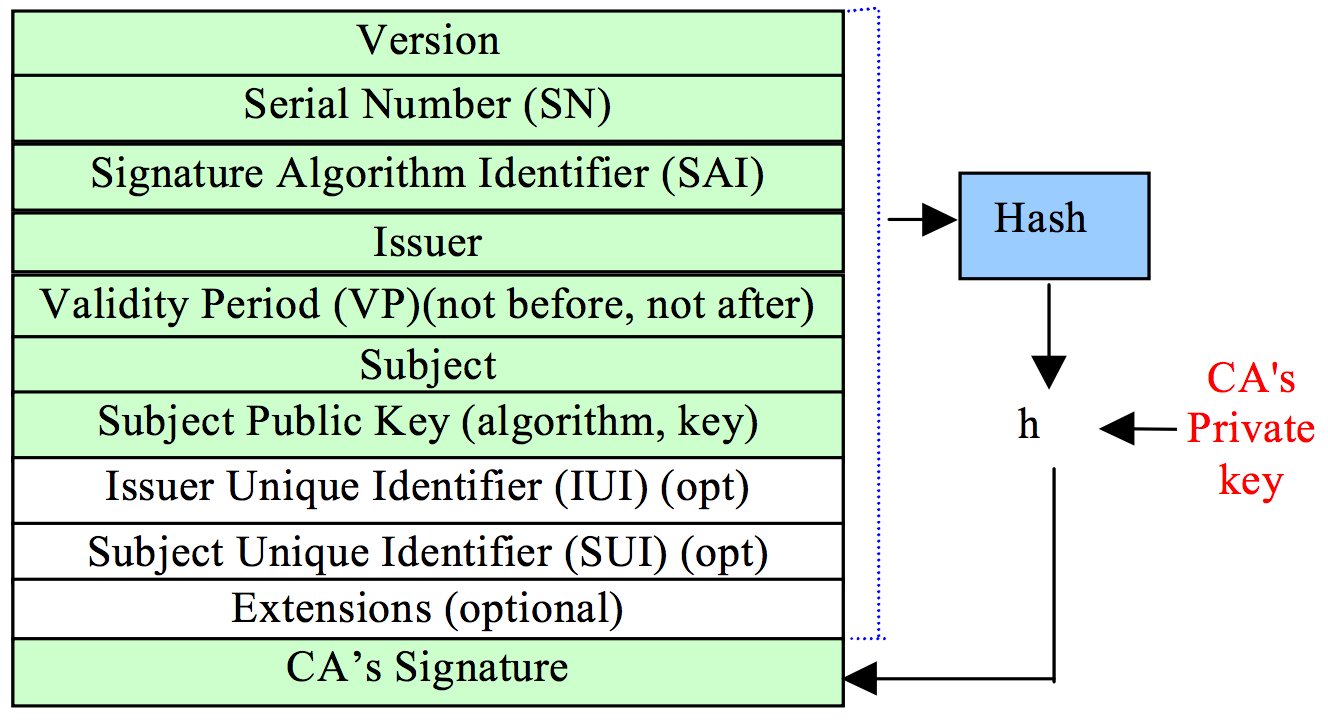
\includegraphics[scale=0.4]{x509.png}
\end{center}
\begin{itemize}
  \item \textbf{Version:} current values are v1, v2 \& v3
  \item \textbf{SN:} a number unique to the issuer (CA)
  \item \textbf{SAI:} identifies the algorithm, such as RSA or DSA, used by the CA to sign the certificate
  \item \textbf{Issuer:} the issuer's name
  \item \textbf{VP:} a range of time when the certificate is valid
  \item \textbf{Subject:} the subject's name
  \item \textbf{SPK:} the subject's public key and parameters, and the identifier of the algorithm with which the key is used.
  \item \textbf{IUI:} to allow the reuse of issuer names over time
  \item \textbf{SUI:} to allow the reuse of subject names over time
  \item \textbf{Ext:} provide a way to associate additional information for subjects, public keys, managing the certification hierarchy and certification revocation lists.
\end{itemize}
The next image is an example:
\begin{center}
  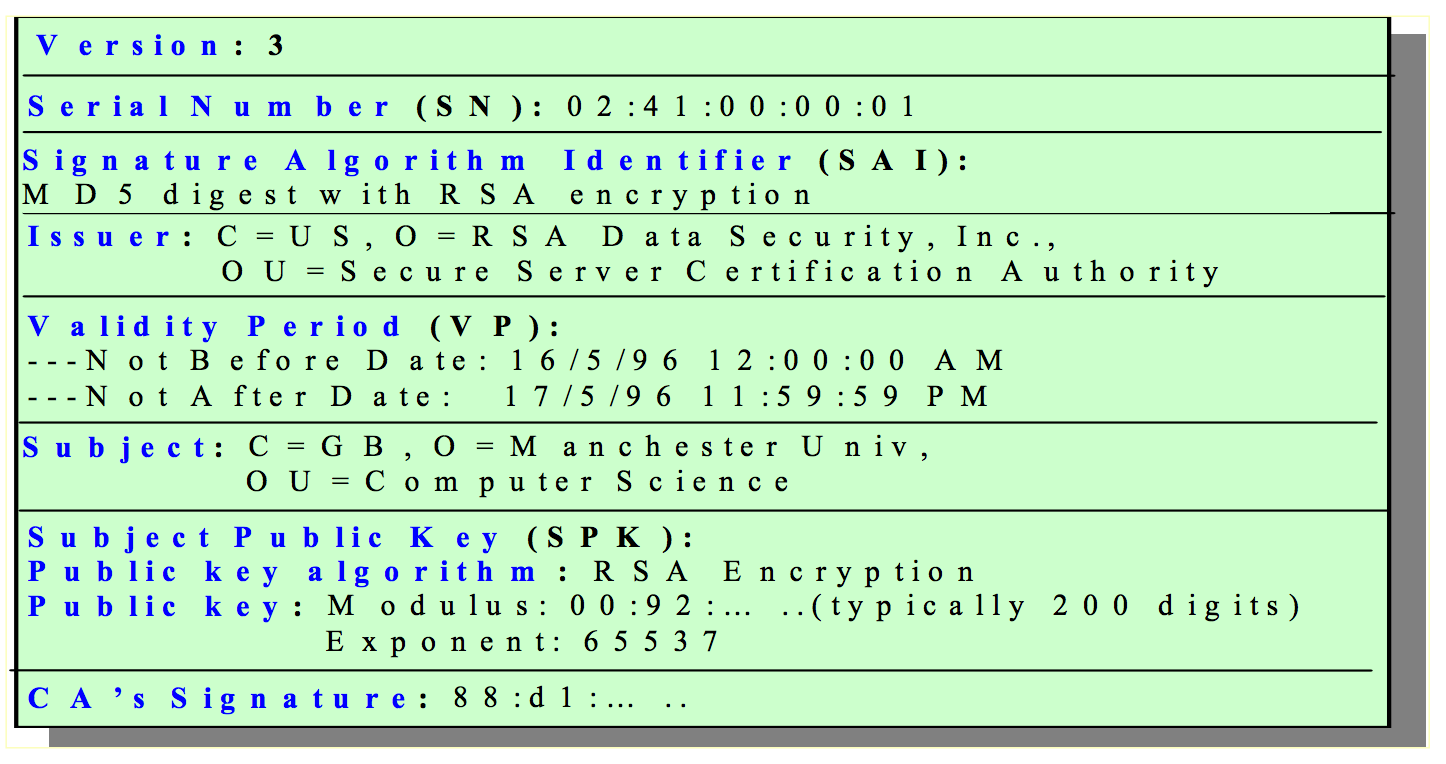
\includegraphics[scale=0.5]{x509-example.png}
\end{center}
\subsection{Certificate Revocation Lists - Why Do We Need It?}
A certificate has a validity period but what if a private key corresponding to a public key certified in a certificate is compromised before the expiration date? We are now vulnerable to repudiation attacks.

Certificate revocation lists is a mechanism to let the world know that a certificate is no longer valid. It is a black list of revoked certificates. A CRL is a data structure, digitally signed by the issuing CA, containing:
\begin{itemize}
  \item Date and time of the CRL publication
  \item Name of the issuing CA
  \item Serial numbers of all the revoked certificates.
\end{itemize}
Using CRL is not that straightforward. The issuing CA needs to keep the CRL up-to-date. A certificate-using application should obtain the most recent CRL and ensure that the certificate serial number is not on the CRL list; in other words, a certificate is said to be valid iff the following verifications are positive:
\begin{itemize}
  \item It has a valid CA signature
  \item It has not expired
  \item It is not listed in the CA's most recent CRL
\end{itemize}
There are also some scalability issues.

\subsection{Top-down Certificate Hierarchy}
In most cases we use more than one CA, as using one root key to sign certificates is too risky if that one key is compromised and also it is not scalable when the user base is large. In some cases, certificate managements may resemble the management structure of an organisation.

The certificate hierarchy starts with a root CA with a root cert/key. They create more keys, sign them with the root key and delegate them to subordinate CAs. Validating a certificate possibly involves validating a chain of certificates (called a chain of trust).

The CA hierarchy would look something like this:
\begin{center}
  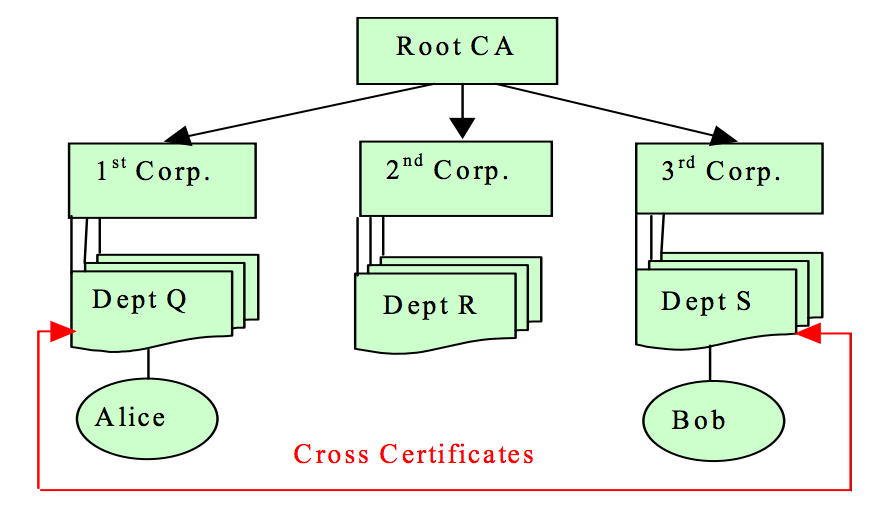
\includegraphics[scale=0.6]{CA-hierarchy.png}
\end{center}
For certificate chain validation we verify that all the digital signatures are signed by all subordinate CAs in a bottom up manner until you reach the root CA's signature, or until you reach a subordinate CA that you can trust. So, for Alice's certificate chain:
\begin{center}
  $\{\text{CERT}_{\text{Alice}}\}S_{\text{DeptQ}} + \{\text{CERT}_{\text{DeptQ}}\}S_{\text{1stCorp}} + \{\text{CERT}_{\text{1stCorp}}\}S_{\text{RootCA}}$
\end{center}
If Bob wishes to authenticate a message signed by Alice, he can proceed `up' the certificate chain until he finds a certificate he can trust.

\subsubsection{Cross Certification}
Cross certification is about expanding trust. If you trust both CA1 and CA2, and a certificate is signed by both, you've got a very high level of trust because two separate entities have verified the certificate.

It has the added bonus of increasing the ease of verification of trust, such as situation were you've got clients that trust CA1 or CA2 but not both. In such a case, you can cross-sign a certificate to be trusted by both. This allows more clients to verify trust without having to distribute separate certificates for different CAs.

Another bonus is in situations where a CA's private key is leaked. Let's say that CA1's key leaks and your certificate is signed by CA1 and CA2. In the wake of the leak, CA1 issue a revokation for it's public key and you can no longer trust anything issued by CA1. However, since your certificate is cross-signed to CA2 as well, any client that trusts CA2 can still maintain a level of trust in your certificate.

\section{Key Management}
Key management is the hardest part of cryptography. How can we generate them so that the can not be easily guessed? How can we securely store keys so that they can not be easily stolen? How could keys be delivered to their intended recipients securely? How could two entities agree on, or establish, a key securely and how are keys revoked and replace?

For symmetrical ciphers, how can we keep the keys secret and for public-key ciphers, how can we ensure that the public keys are trustworthy?

Below is a table which shows the number of possible keys given various constraints as well as the time it would take to crack them given $10^{6}$ attempts per second:
\begin{center}
  \begin{tabular}{lll}
    \hline
    & 6-bytes & 8-bytes \\
    \hline
    Lowercase letters (26) & $3.1 * 10^{8}$ & $2.1 * 10^{11}$ \\
    & 5 min & 2.4 days \\
    Lowercase letters \& digits (36) & $2.2 * 10^{9}$ & $2.8 * 10^{12}$ \\
    & 36 mins & 33 days \\
    Alphanumeric characters (62) & $5.7 * 10^{10}$ & $2.2 * 10^{14}$ \\
    & 16 hours & 6.9 years \\
    Printable characters (95) & $7.4 * 10^{11}$ & $6.6 * 10^{15}$ \\
    & 8.5 days & 210 years \\
    ASCII characters (128) & $4.4 * 10^{12}$ & $7.2 * 10^{16}$ \\
    & 51 days & 2300 years
  \end{tabular}
\end{center}

\subsection{Key Generation}
Good keys are random numbers, a sequence of numbers where an observer can not predict one of the numbers given all of the others in the sequence. Ordinary random number generation functions e.g. \texttt{java.util.Random}, may not be good enough for this. A reliable random source, or a cryptographically secure pseudo-random number generator, e.g. \texttt{SecureRandom} class in \texttt{java.security} package should be used.

Some pseudo-random numbers are generated from a strong mixing function that takes two or more inputs that have some randomness (e.g. CPU load, arrival times of network packets), but produces an output bit of which depends on some nonlinear function of all the bits of the inputs. Cryptographic hashing functions and encryption algorithms (e.g. MD5, SHA and DES) are all examples of the strong mixing function.

\subsection{Key Storage}
You must protect the key to the same degree as all the data it encrypts. Attackers may defeat access control mechanisms, so you should encrypt the file containing the key. Ideally, a key should never appear unencrypted outside the encryption device.

The key may be resident in memory, so attackers may be able to read it if they could get access to the machine. Therefore, you can use a physical token to store the key such as a smart card, and protect the token with a PIN number. The card could be stolen so therefore you can split they key into two halves and store one half on the card and the other in the machine.

\subsection{Session Key Establishment}
The more often a symmetric key is used, the more likely it is to be cracked. Therefore we should generate and use a symmetric key for one session only. It is desirable to use different session keys in different sessions as this can:
\begin{itemize}
  \item Limit available ciphertexts for cyptanalysis
  \item Limit exposure (both in time period and amount of data) in an event of key compromise
  \item Avoid long-term storage of a large number of secret keys by only creating them when needed.
\end{itemize}
To establish a session key, one way it to use a key agreement protocol. A shared secret is derived by the parties as a function of information contributed by each, such that no party can predetermine the resulting value (Diffie-Hellman protocol).

Another way is to use key transportation protocols. If we're not using a public-key cipher session keys are generated and distributed with the help of a third party (Needham-Schroeder protocol). If we're using a public-key cipher one party creates a session key and securely transfers it to the other party using the recipients public key.

With this being said, there are other issues that should be considered. \\
\textbf{Entity and key authentication:}
\begin{itemize}
  \item Assurance: no other party could gain access to the established session key.
  \item Key confirmation: asking the other entity to demonstrate that he has the knowledge of the key by either producing a one way hash value of the key or encrypting some known data (e.g. nonce) with the key.
\end{itemize}
\textbf{Key freshness:} assurance that the key is fresh i.e. not used before.

\subsection{Diffie-Hellman Protocol}
BH was the first public-key algorithm ever invented back in 1976. The DH key exchange protocol allows two parties who have never met before to exchange protocol messages in public and collectively generate a key that is private to them, and none of the parties could predetermine the key.

Its security is based on the difficulty of calculating discrete logarithms in a finite field:
\begin{itemize}
  \item Given integers $y$ and $g$ and prime number $n$, compute $x$ such that $y = g^{x} \Mod n$.
  \item Solutions known for small $n$.
  \item Solutions computationally infeasible as $n$ grows large.
\end{itemize}
Assuming that two parties, Alice and Bob, take part in the exchange. They agree on two large integers, $g$ and $n$. $n$ is a prime number that serves as the modulus and $g$ is a random number that serves as the basis with $1 < g < n$. $g$ and $n$ do not have to be secret. Alice has a private key $X_{a}$ and a public key $Y_{a}$ and so does Bob, $X_{b}$ and $Y_{b}$. The image below shows how the algorithm works:
\begin{center}
  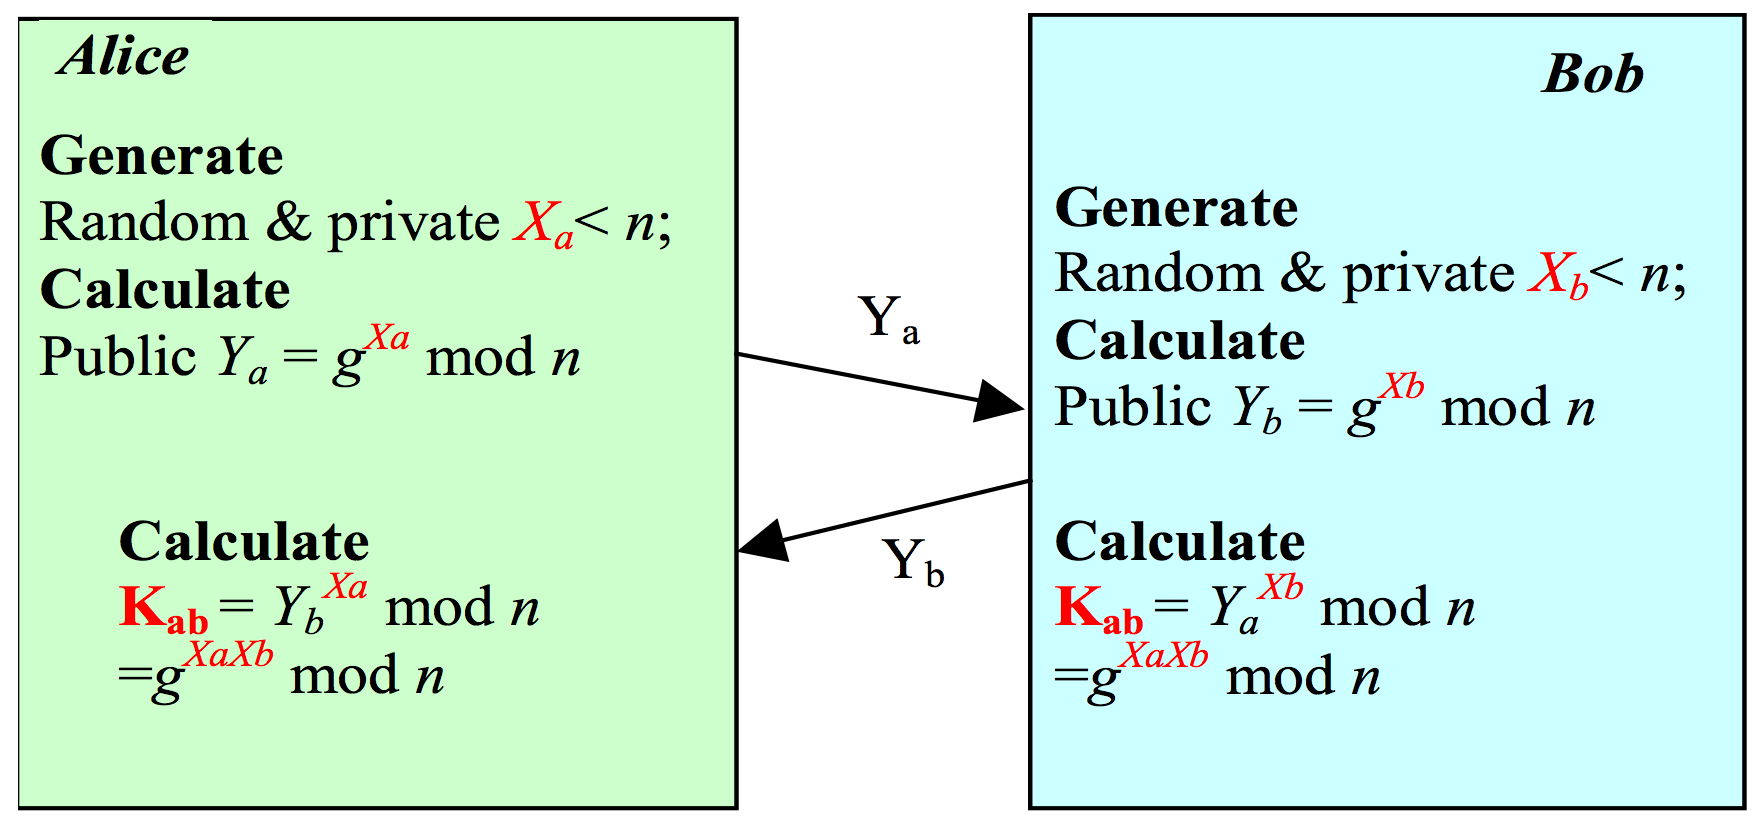
\includegraphics[scale=0.3]{dh.png}
\end{center}
This resists passive attacks such as eavesdropper as calculating a discrete logarithm is a computationally hard problem. There is one problem though. Neither party knows who it shares the secret with so it is vulnerable to active man-in-the-middle attacks.

\subsection{Distribution Without Use of PKC}
\textbf{Approach one:} Given $n$ users, we provide $n(n-1)/2$ keys. The problem with this is that as $n$ increases, the number of keys needed becomes untenable for everyone, the $n^{2}$ problem.

\textbf{Approach two:} Use a key distribution centre (KDC) or server which also includes a key hierarchy where there are master keys (for long-term use) and session keys.

A unique master key, shared between either a pair of users or a KDC, is for session key distribution. The session key is to secure the communication. The advantage of using approach two is that it reduces the scale of the problem. The $n^{2}$ problem is reduced to an $n$ problem therefore making the system more scalable.

The disadvantage of approach two is that there is a need to trust the KDC. The KDC has enough information to impersonate anyone to anyone. If the system is compromised, all the resources in the system are vulnerable.

\subsubsection{The Needham-Schroeder Protocol}
The Needham-Schroeder protocol uses approach two that's mentioned above. Both parties, $A$ and $B$ share a secret key with the KDC, $K_{a}$ and $K_{b}$. $A$ and $B$ wish to establish a secure communication channel, i.e. establish a shared one-time session key $K_{ab}$ for use between $A$ and $B$.

$N_{a}$ and $N_{b}$ are nonces (random challenges), generated by $A$ and $B$ respectively, to keep the request fresh. Below is a diagram showing how the Needham-Schroeder protocol works.
\begin{center}
  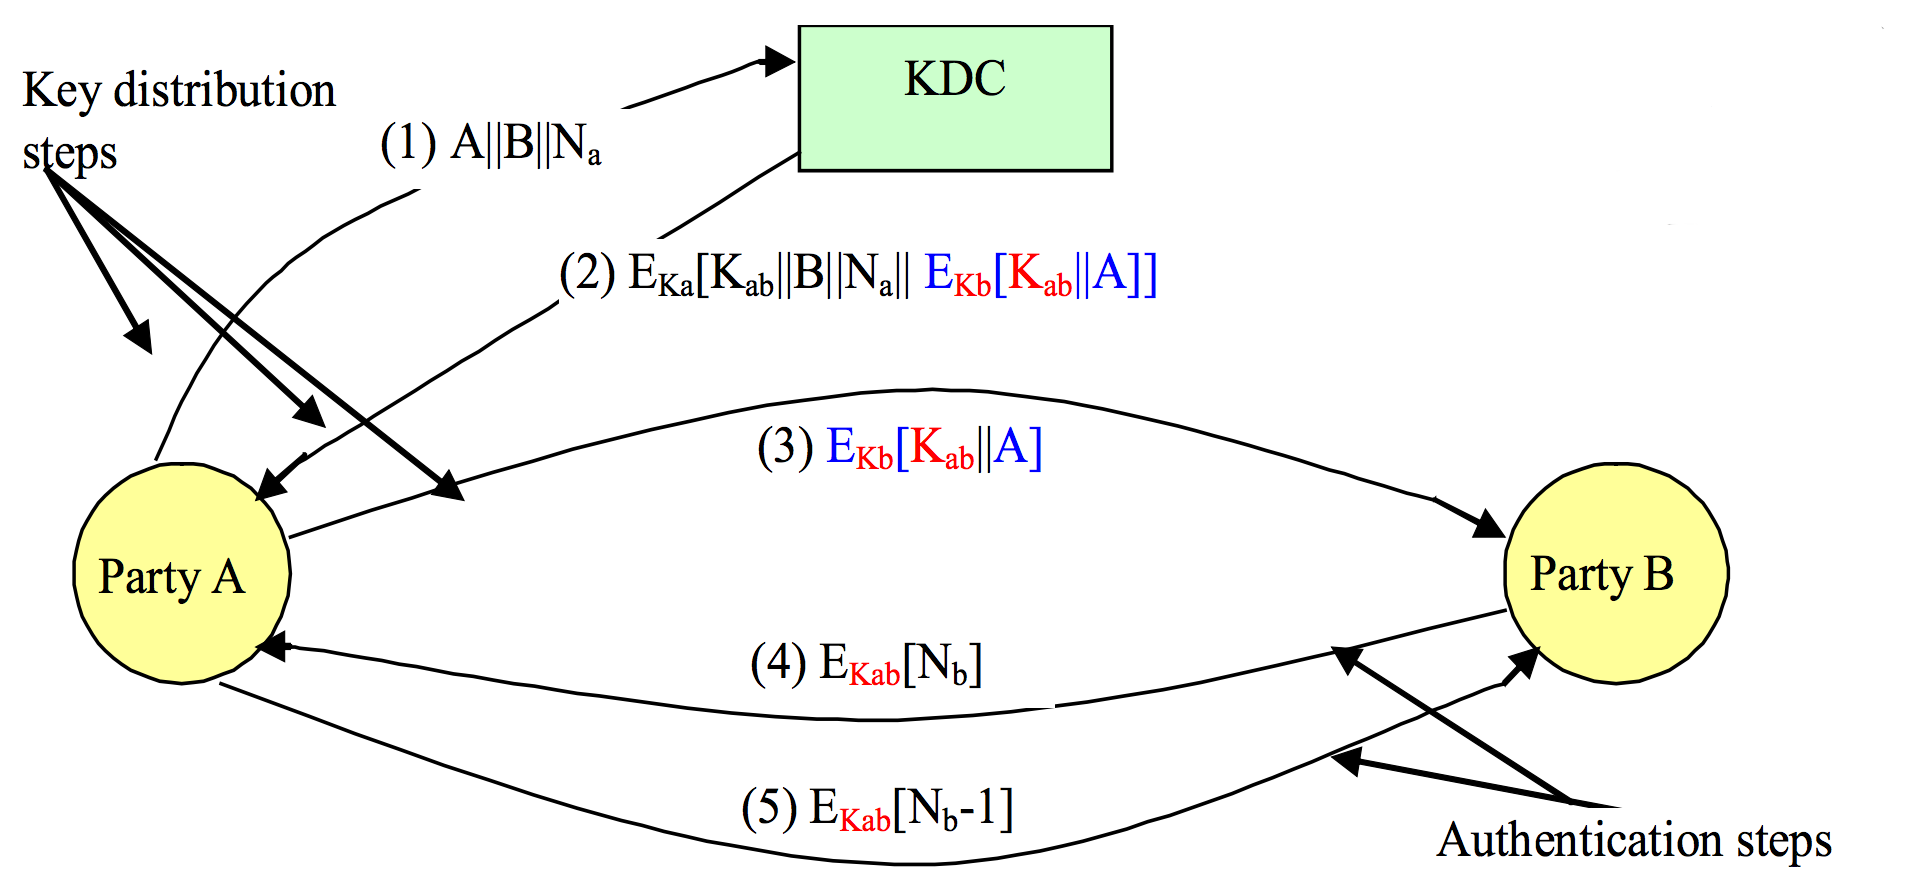
\includegraphics[scale=0.4]{nsp.png}
\end{center}

\begin{enumerate}
  \item $A$ sends a request to KDC for a session key to establish a secure channel with $B$.
  \item KDC generates a random number $K_{ab}$, and replies with the response containing the session key $K_{ab}$, the original request from $A$ matching the response with the request and an item (the session key and $A$'s identity) which only $B$ can view.
  \item $A$ forwards the item to $B$. At this point, the session key is securely delivered to $A$ and $B$, and they may begin secure communication.
  \item $B$ sends a nonce $N_{b}$ to $A$ encrypted using the new session key.
  \item $A$ responds with $N_{b}-1$.
\end{enumerate}
Steps 4 and 5 assure $B$ that the message received in 3 was not a reply, i.e. to authenticate $A$.

\subsection{Distribution using PKC}
\subsubsection{Two-passes Method}
In this method there is secret key distribution with mutual authentication using a public key cryptosystem and timestamps:
\begin{center}
  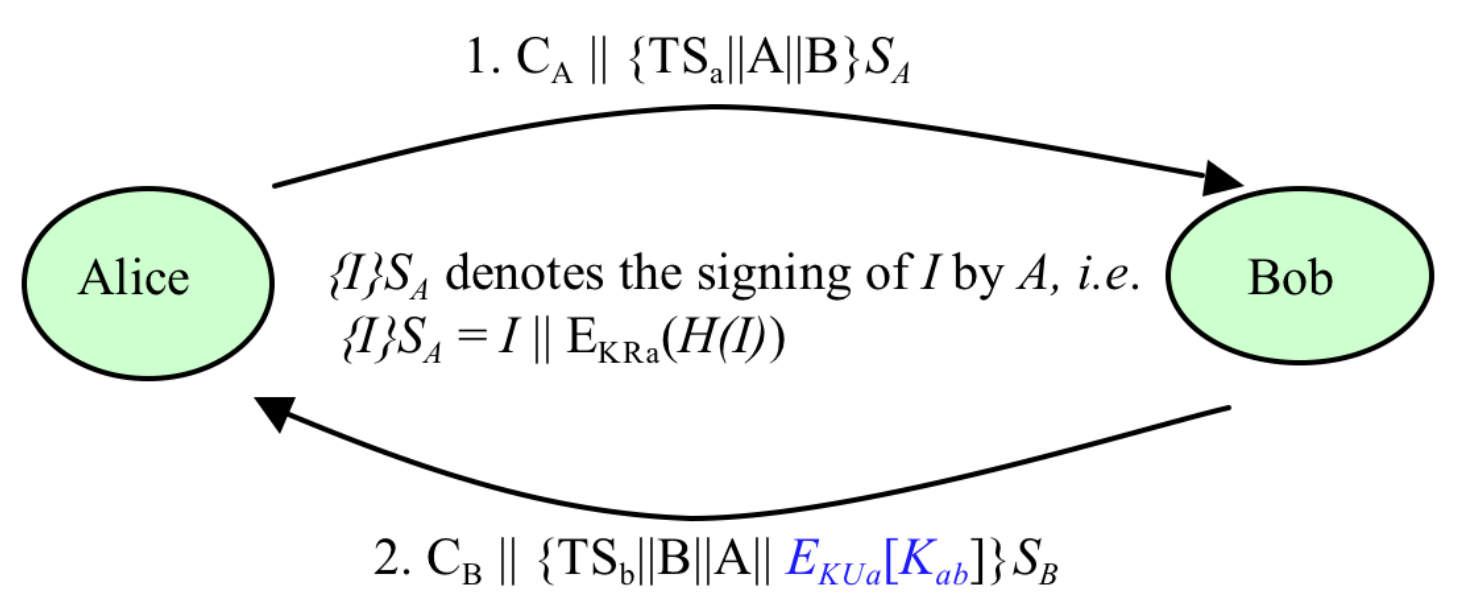
\includegraphics[scale=0.4]{two-passes.png}
\end{center}
\subsubsection{Three-passes Method}
In this method there is symmetrical key distribution with mutual authentication using digital signatures and nonces:
\begin{center}
  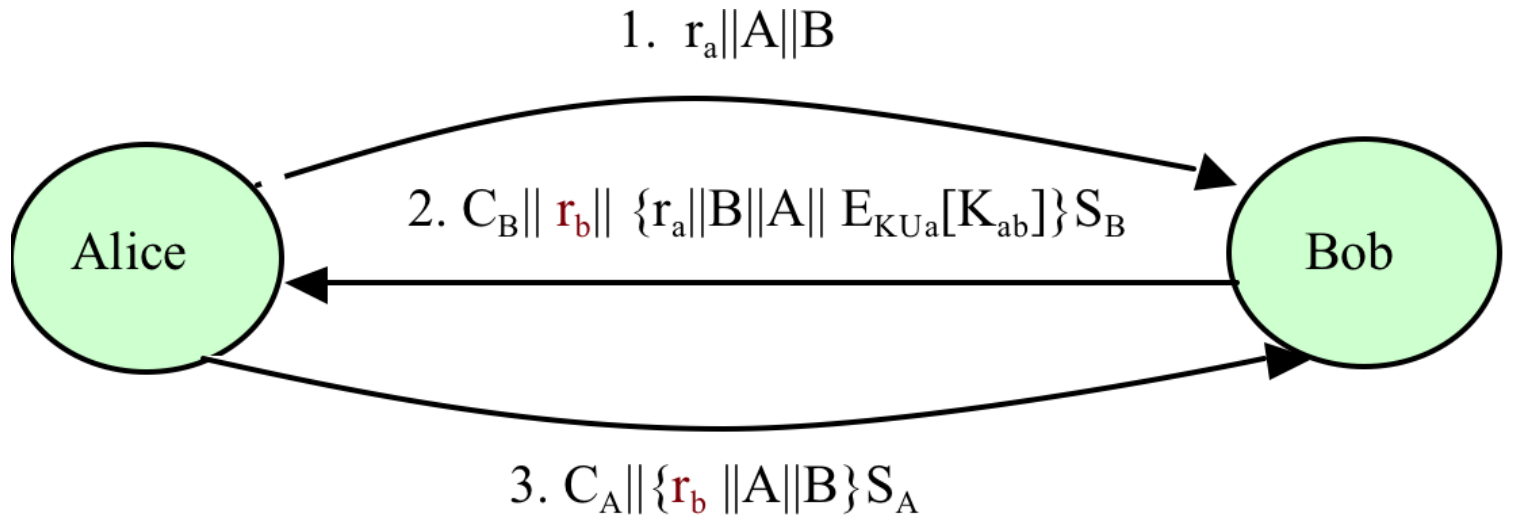
\includegraphics[scale=0.4]{three-passes.png}
\end{center}

\subsection{Summary of Secret Key Establishment Protocols}
\begin{center}
  \begin{tabular}{|p{2.5cm}|p{2.5cm}|p{2.5cm}|p{4cm}|p{2cm}|}
    \hline
    Protocols & ThirdParty & Timestamps & EntityAuth & Messages \\ \hline
    Diffie-Hellman & No & No & None & 2 \\ \hline
    Needham-Schroeder & KDC (online) & No & Symmetric encryption & 5 \\ \hline
    Kerberos & KDC (online) & Yes & Symmetric encryption & 4 \\ \hline
    X.509 (2 pass) & CA (offline) & Yes & mutual & 2 \\ \hline
    X.509 (3 pass) & CA (offline) & No, but with nonce & mutual & 3 \\
    \hline
  \end{tabular}
\end{center}

\section{Authentication}
Some methods for user identification/authentication are:
\begin{itemize}
  \item Where you are: location authentication based on IP addresses etc.
  \item Something you know: passwords, PIN.
  \item Something you have: keys, smart cards etc.
  \item Something you are: biometrics, voice recognition.
\end{itemize}
These methods combined may be used for a higher level of assurance.

\subsection{Password-based Authentication}
The UNIX system chooses not to store plaintext passwords, rather it stored encrypted/hashed passwords in the password file. Storing passwords for all the system users plainly visible in a password file is vulnerable to theft and accidental disclosure. The hashing algorithm is a one-way function, called \texttt{crypt()} that is modified based upon the DES algorithm. It uses salt to make the DES based one-way function different from DES and to make dictionary attacks harder to succeed. The crypt algorithm:
\begin{itemize}
  \item Using DES with the first 7 bits of the first 8 characters of password as the key.
  \item Iterated 25 times on constant string 0s; making the process slower.
  \item Using salt to perturb the DES algorithm, so that DES chip can not be used to (dictionary) attack the algorithm. It makes pre-compiled dictionary attacks harder (by a factor of 4096) and it prevents an identical password from producing the same encrypted password.
  \item The final 64 bits are unpacked into a string of 11 printable characters, called \textit{the encrypted password}
\end{itemize}
Most of today's implementations support MD5 in addition to the legacy DES-based \texttt{crypt()} function.

When a user have an account created or they change their password, the \texttt{/bin/password} program:
\begin{itemize}
  \item Selects a salt based on the time of day; the DES salt is a 12-bit number, between 0 and 4095, that is converted into a two-character string and is stored in the \texttt{/etc/passwd} file along with the encrypted password.
  \item The password is used as the encryption key to encrypt a block of zero bits using \texttt{crypt()} to generate the encrypted password.
\end{itemize}
When a user tries to log in, the program \texttt{/bin/login} takes the password the user typed, and the salt from the password file, to generate a fresh encrypted password, and compares the newly generated one with the one stored in the \texttt{/etc/passwd} file. If the two encrypted results match, the system lets you in.

In the UNIX password file, each entry in the file is for one account and has several fields separated by colons, an image of this is below:
\begin{center}
  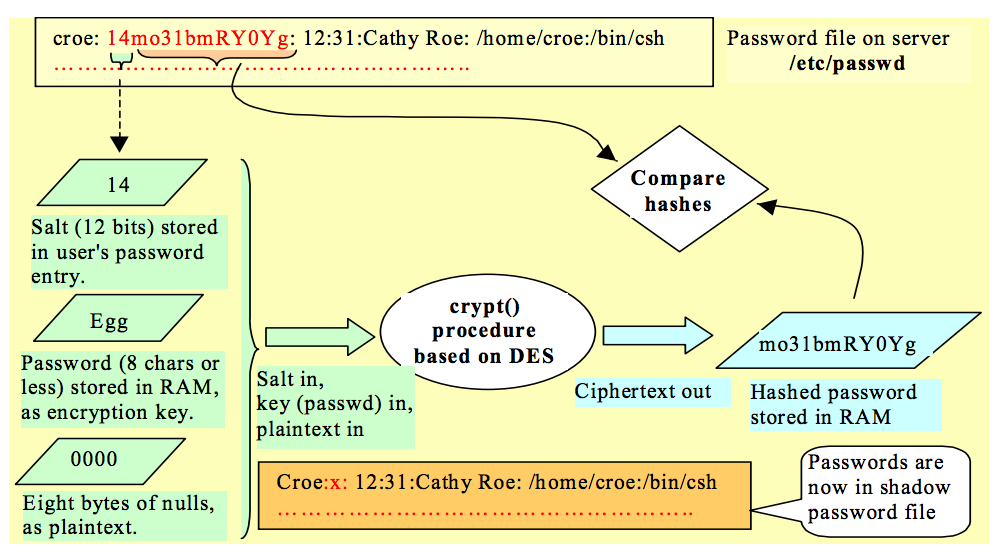
\includegraphics[scale=0.6]{unix-pass.png}
\end{center}
\begin{itemize}
  \item User name (croe)
  \item Password (14mo31bmRY0Yg): the hashed password preceded by a salt value (14) to be used with the password.
  \item User ID (UID=12): a number assigned to this user name for system use in identifying the account.
  \item Group ID (GID=31): a number for the user's group.
  \item Home directory (/home/croe)
  \item Shell (/bin/csh): the user's default shell program.
\end{itemize}
This design causes a problem though. \texttt{/etc/passwd} needs to be accessed by processes, so the solution above would allow anyone to copy the file and to crack the passwords at his/her leisure. The countermeasure to this is the a shadow password file, \texttt{/etc/shadow} is used which stores the real passwords and is put in an area accessible only to the root account.

Another problem is that an attacker can eavesdrop on a network to get your login ID and encrypted password and later replay it to gain access to the network - the replay attack. In order to perform this attack the attacker needs to:
\begin{itemize}
  \item Modify the client/logon software so that it does not encrypt the encrypted password but rather replay it directly.
  \item Eavesdrop on the network
\end{itemize}
Usually we assume that the LAN is secure and you do not bring your own client software in so we tend to overlook this problem in a LAN environment.

\subsubsection{One-Time Passwords}
These are passwords that can only be used once that therefore thwart sniffing and replay attacks. Below are some approaches to one-time passwords:
\begin{itemize}
  \item random number based OTP.
  \item Clock-based OTP (need token). The clock has to be reliable and secure. The clocks between the entities must be synchronised.
  \item Counter-based OTP (need token).
  \item If a hard token is used, then the token should be locked with a PIN or password.
\end{itemize}

\subsection{CHAP (Challenge-Handshake Authentication Protocol)}
The CHAP authenticates a user or network host to an authenticating entity for example an ISP, VPN server, wireless access point etc.

CHAP provides protection against replay attacks by the peer through the use of an incrementally changing identifier and of a variable challenge value. CHAP requires that both the client and server know the plaintext of the secret, although it is never sent over the network. Thus, CHAP provides better security as compared to Password Authentication Protocol which is vulnerable for both these reasons.
\begin{enumerate}
  \item After completion of the link establishment phase, the authenticator sends a challenge message to the peer.
  \item The peer responds with a value calculated using a one-way hash function on the challenge and the secret combined.
  \item The authenticator checks the response against its own calculation of the expected hash value. If the values match, the authenticator acknowledges the authentication; otherwise it should terminate the connection.
  \item At random intervals the authenticator sends a new challenge to the peer and repeats steps 1 through 3.
\end{enumerate}
\begin{center}
  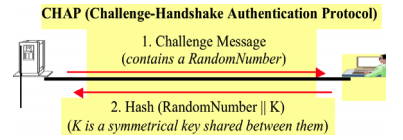
\includegraphics[scale=0.6]{chap.png}
\end{center}

\subsection{PIN protected OTP}
This method uses a PIN to unlock a token, i.e. when a PIN is entered, the token compares the PIN typed in against an internal copy. If positive, the token will compute the OTP using the reading from the clock or counter embedded in the token + the base secret. If repeated PIN entries are wrong, the token takes steps to resist a PIN guessing attack.

\subsection{Smart-card-based Authentication}
A smart-card is an authentication token that a person carries around with them. Some advantages are:
\begin{itemize}
  \item Unlike memory cards, they can do more than just containing some secret information; they can perform simple crypto operations.
  \item Support mobility, can `memorise' your secret, and can provide two factor authentication.
\end{itemize}
And some disadvantages:
\begin{itemize}
  \item Smart-cards require a special hardware reader on every access device, which may be expensive and requires standardisation.
  \item They are subject to theft, so used in conjunction with some other authentication mechanisms such as PIN/password.
\end{itemize}

\subsection{Challenge-Response Using PKC}
The previous protocol requires a shared symmetric key; what if you have not already established that trust relationship? We authenticate using public key technique with a nonce.
\begin{center}
  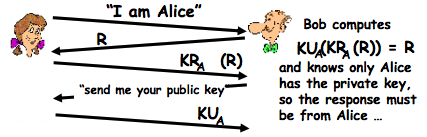
\includegraphics[scale=0.7]{crpkc.png}
\end{center}
The security hole here is a man-in-the-middle attack:
\begin{center}
  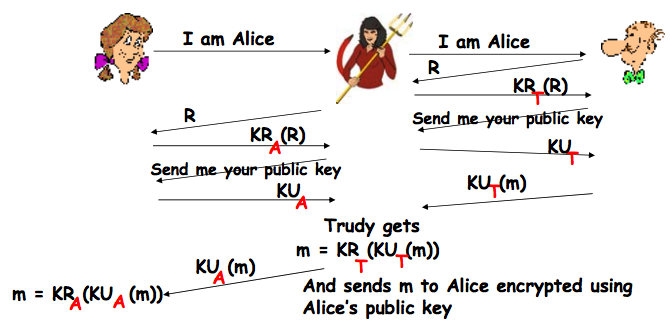
\includegraphics[scale=0.5]{crpkc-mitm.png}
\end{center}

\subsection{X.509 Certificate-based Authentication Service}
X.509 defines a framework - a system to enable the validation of, and to give legal meaning to, digital signatures (which require the use of hash functions). It allows mutual authentication using public-key technology - digital signatures are digital certificates. It doesn't dictate the use of a specific public-key cryptographic algorithm, but recommends RSA, nor does it define a specific hash algorithm. It's used in S/MIME, IP Security, SSL/TLS and SET. Below is an image showing the authentication process:
\begin{center}
  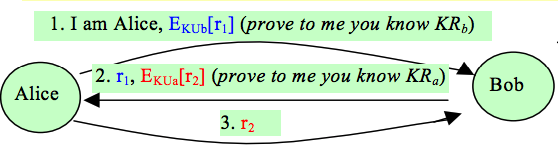
\includegraphics[scale=0.5]{x509-auth.png}
\end{center}
As only $B$ can decrypt the random number (nonce), $r_{1}$, correctly, message (2) authenticates $B$ to $A$. Message (3) authenticates $A$ to $B$. Three messages are needed for mutual authentication between two parties. This is called challenge-response authentication method.

\subsubsection{X.509 - Authentication Using Digital Signatures}
\begin{center}
  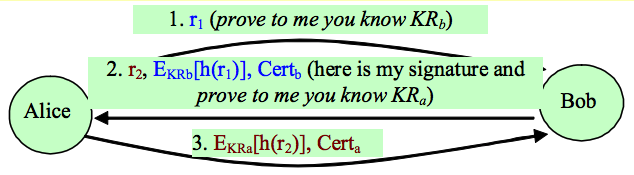
\includegraphics[scale=0.5]{x509-auth-sig.png}
\end{center}
As only $B$ can generate the rightful signature, message (2) authenticates $B$ to $A$. Message (3) authenticates $A$ to $B$. This is also called challenge-response authentication method.

\subsection{Enterprise authentication}
We have seen what it's like for single systems as shown earlier but what about when we have more systems and more passwords? For this we can use central authentication for a number of systems in an organisation. We let one authority (usually called a security server) at an organisation/site manage your passwords instead of each computer having its own. By this, we can enforce organisation wide security policies, including authentication, authorisation and accounting (i.e. the AAA services). A number of systems exist such as Radius and Kerberos.

The security server is responsible for providing AAA services to edge devices such as VPN servers and wireless access points.

\subsubsection{RADIUS}
The image below is an overview of how the RADIUS authentication system works:
\begin{center}
  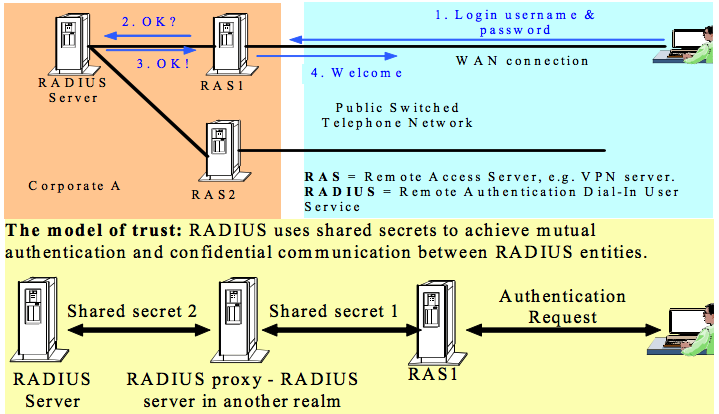
\includegraphics[scale=0.5]{radius-overview.png}
\end{center}
The next is how simple user authentication and authorisation works with RADIUS:
\begin{center}
  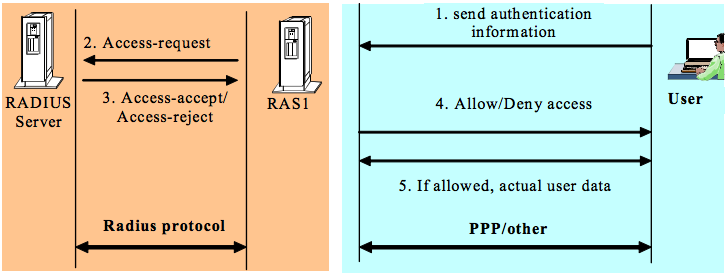
\includegraphics[scale=0.5]{radius-user-auth.png}
\end{center}
And finally how challenge-response authentication and authorisation works using RADIUS:
\begin{center}
  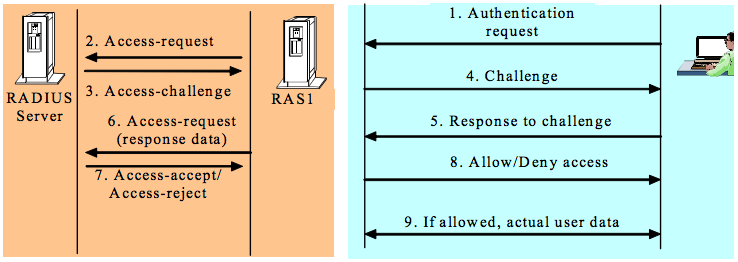
\includegraphics[scale=0.5]{radius-cr-auth.png}
\end{center}
In general the RADIUS protocol works in the following way:
\begin{itemize}
  \item The client forwards the user access request to a RADIUS server.
  \item Server replies with reject access or allow access based on a user supplied password/credential.
  \item Server challenges when challenge-response protocol is used.
  \item If challenge-response is used, client forwards challenge to the user and the user sends their response to the client and then the client onto the server.
  \item One RADIUS server may act as a client to another RADIUS server for consultation.
\end{itemize}

\section{Virtual Private Networks}
A VPN is a security solution, making use of tunnelling, encryption, authentication, and access control technologies to allow you to achieve private communication over public networks such as the Internet.

Tunneling includes \textbf{encapsulation}, \textbf{transmission} and \textbf{decapsulation}; encapsulation is to wrap data with a header that provides routing information allowing it to transmit across the Internet to reach its destination so as to emulate a dedicated point-to-point link. For example, in IP-in-IP encapsulation, IP packets are encapsulated in another IP packet.

VPN routers (or VPN gateways) are located at the corporate network perimeter; they perform tunneling, authentication and data encryption/decryption. They can be categorised as \textbf{standalone} or \textbf{integrated}:\\
\textbf{Standalone}: VPNs incorporate purpose-built devices.\\
\textbf{Integrated}: Implementations add VPN functionality to existing devices such as routers, firewalls:
\begin{itemize}
  \item Router based VPNs add encryption support to existing routers and can keep the upgrade costs of VPN low.
  \item Firewall based VPNs are a workable solution for small networks with low traffic volume.
\end{itemize}
A VPN client is:
\begin{itemize}
  \item Software used for remote VPN access.
  \item Creates a secure path from the remote client computer to a VPN gateway.
  \item Can be loaded onto an individual computer requesting remote access \textbf{or} a router that establishes a peer-to-peer VPN connection.
\end{itemize}
During tunnel setup, the devices on each side of the tunnel agree on the details of authentication and encryption.
\begin{itemize}
  \item Authentication is for identifying VPN users and devices and for ensuring the authenticity of data.
  \item Encryption is for protecting the confidentiality of data while in transit across the Internet.
\end{itemize}
Below is a table showing different VPN types:
\begin{center}
  \begin{tabular}{|p{2.5cm}|p{3cm}|p{2.5cm}|p{3cm}|}
    \hline
    Types & Applications & Alternatives & Benefits \\ \hline
    Remote access VPN & Remote connectivity & Dedicated dial ISDN & Ubiquitous access, lower cost \\ \hline
    Intranet VPN & Site-to-site, internal connectivity & Leased line & Extended connectivity, lower cost \\ \hline
    Extranet VPN & B2B, external connectivity & Fax, snail post & Facilitates eTransaction and eCommerce \\
    \hline
  \end{tabular}
\end{center}
We need VPNs to protect us against security risks on the internet such as:
\begin{itemize}
  \item Loss of privacy (packet sniffing).
  \item Loss of data integrity - data can be modified maliciously or accidentally.
  \item Identity spoofing.
  \item Denial of Service attacks.
\end{itemize}
There are multiple ways of implementing a VPN. PPTP is based upon PPP (point-to-point protocol). L2TP 9Layer 2 tunnelling protocol) is an extension or enhanced version of PPTP; often used together with IPSec and then there is just normal IPSec. Although IPSec has become the de facto standard for LAN-WAN-LAN VPNs, PPTP and L2TP are heavily used for single client to LAN connections. Therefore, many VPN products support IPSec, PPTP and L2TP.

\section{IPSec}
IPSec operates at the IP layer. It provides security protection:
\begin{itemize}
  \item For the transport layer, including all TCP and UDP, traffic.
  \item For all other traffic carried in the data field of the IP packet e.g. ICMP messages.
  \item Also for IP packets (IPv4 and IPv6) when using tunnel mode.
\end{itemize}
This protection is transparent, i.e. there is no need to modify applications or transport-layer protocols to work with IPSec, and can be applied to all the application-level programs.

\subsection{Security Association (SA) And Session Keys}
A security association refers to a set of attributes negotiated between two end-points for the protection of IP traffic for the SA. Some of the attributes are:
\begin{itemize}
  \item Authentication mechanism e.g. HMAC
  \item Encryption algorithm e.g. DES
  \item Algorithm mode e.g. CBC
  \item A shared session key
  \item Initialisation vector
\end{itemize}
This system is unidirectional, so for two-way secure exchange two SAs are needed. An SA is uniquely identified by:
\begin{itemize}
  \item A random 32-bit value SPI (secure parameter index)
  \item Destination IP address
  \item An identifier of the security protocol (AH or ESP)
\end{itemize}
Session key establishment can either be managed manually or automatically. If you choose to establish them manually you have to manually configure the keying material and SA data for each system. This is practical in small, static environments an does not scale well.

For automated key management there is ISAKMP (Internet SA Key Management Protocol) which defines procedures and packet formats to establish, negotiate, modify and delete SA. There is also the IKE (Internet Key Exchange) which provides facilities to negotiate and derive keying material for establishing a session key:
\begin{itemize}
  \item DH-DSA: using Diffie-Hellman key agreement for deriving key material between peers on a public network, and DSA to sign the DH exchanges to counter the man-in-the-middle attack.
  \item Public key cryptography: using recipients public key for secure session key transportation.
\end{itemize}
Below is a diagram which illustrates the process of establishing an SA and session key:
\begin{center}
  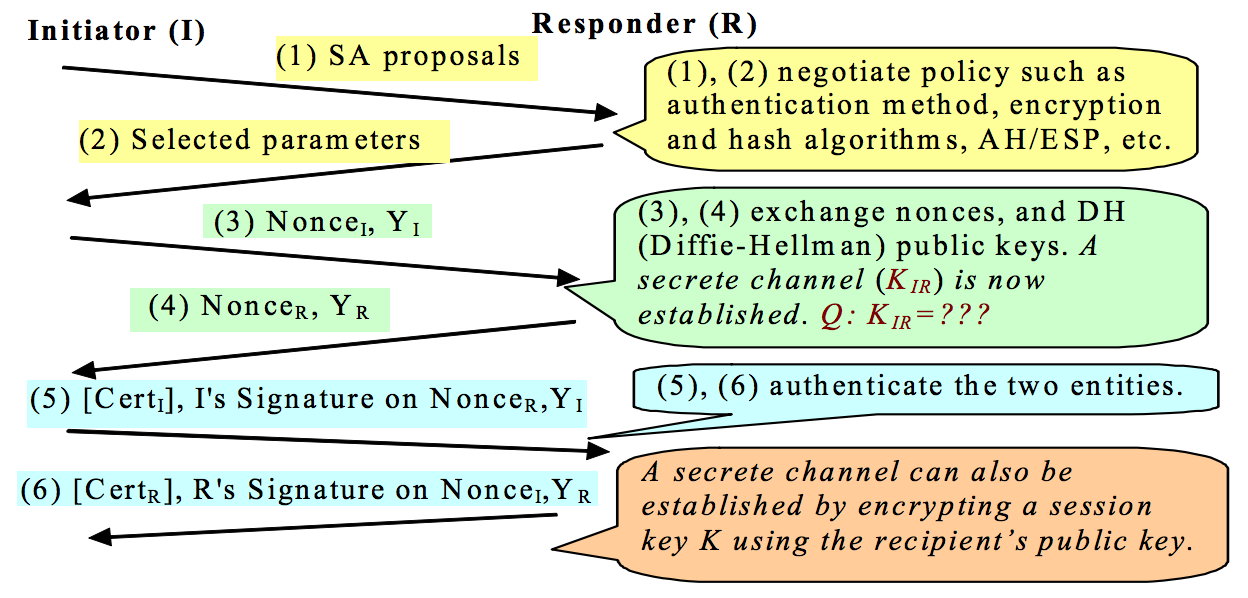
\includegraphics[scale=0.6]{sa-sk-establishment.png}
\end{center}

\subsection{Authentication Methods}
ISAKMP/IKE supports multiple \textbf{authentication} methods. Scheme one in symmetric key cryptography:
\begin{itemize}
  \item The same key is pre-installed on each host.
  \item The peers authenticate each other by computing and sending a keyed hash of data that includes the pre-shared keys.
\end{itemize}
The second is public key cryptography:
\begin{itemize}
  \item Each party generates a pseudo-random number (nonce) and encrypts it and its ID using the other party's public key.
  \item The ability to decrypt the data with the local private key authenticates the parties to each other.
  \item The method requires the ability to generate random numbers, and perform public-key encryption/decryption.
  \item It does not provide non-repudiation.
  \item Currently only RSA is supported.
\end{itemize}
The third is digital signature:
\begin{itemize}
  \item Each device signs some data contributed by the other entity.
  \item This method is similar to scheme two, except that it provides non-repudiation.
  \item Both RSA and DSS are supported.
\end{itemize}
Once SA(s) is negotiated and session key established, packets are forwarded using traffic protocols, AH and/or ESP.

IPSec (AH and ESP) may be employed in one of the two ways. \textbf{Transport} and \textbf{tunnel} modes (or a combination of them).

\subsection{Transport Mode}
Transport mode is only applicable to host implementations and it protects the IP payload (the data). The payload is encapsulated by the IPSec headers and trailers. The original IP headers remain intact, except that the IP protocol field is changed to ESP or AH, and the original protocol value is save is the IPSec trailer to be restores when the packer is decrypted.

Transport mode is usually used when another tunneling protocol is used to first encapsulate the IP data packet, then IPSec is used to protect the tunnel packets.

The packet diagram below illustrates IPSec transport mode with ESP header
\begin{center}
  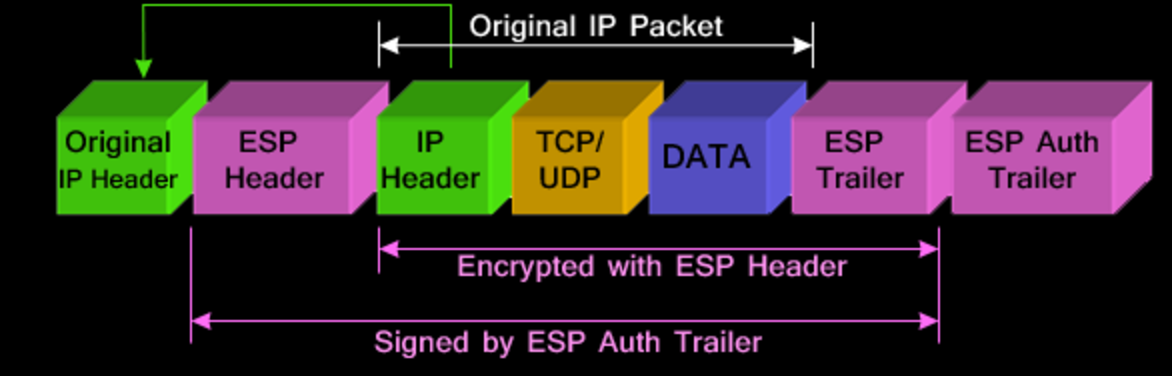
\includegraphics[scale=0.6]{ipsec-transport.png}
\end{center}

The packet diagram below illustrates IPSec transport mode with AH header
\begin{center}
  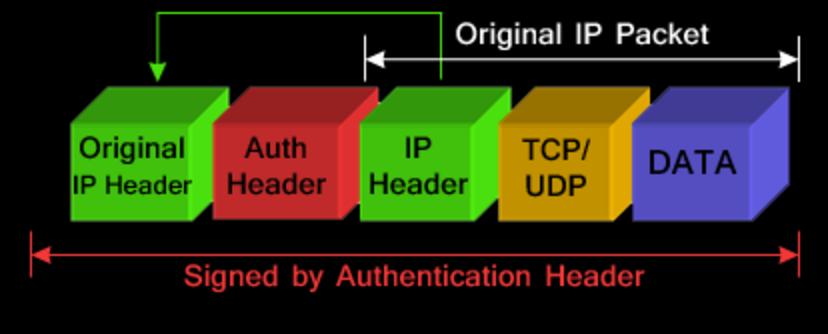
\includegraphics[scale=0.6]{ipsec-transport-ah.png}
\end{center}

\subsection{Tunnel Mode}
Tunnel mode is employed in either hosts or security gateways; the entire original IP datagram is protected (it becomes the payload in a new IP packet). It allows a network device to act as an IPSec proxy performing IPSec processing on behalf of the hosts. This method protects against traffic analysis.

In tunnel mode, an IPSec header is inserted between the IP header and the upper layer protocol. Between AH and ESP, ESP is most commonly used in IPSec VPN tunnel configuration.

The packet diagram below illustrates IPSec tunnel mode with ESP header.
\begin{center}
  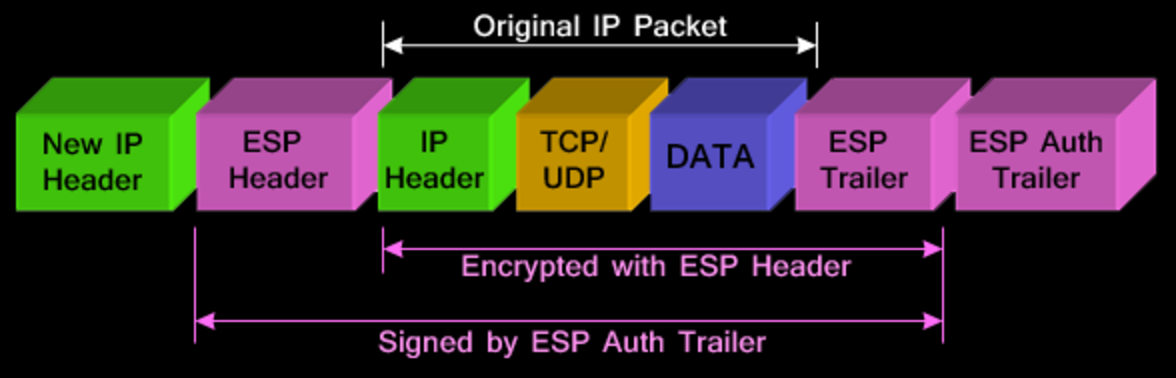
\includegraphics[scale=0.6]{ipsec-tunnel.png}
\end{center}

The packet diagram below illustrates IPSec tunnel mode with AH header.
\begin{center}
  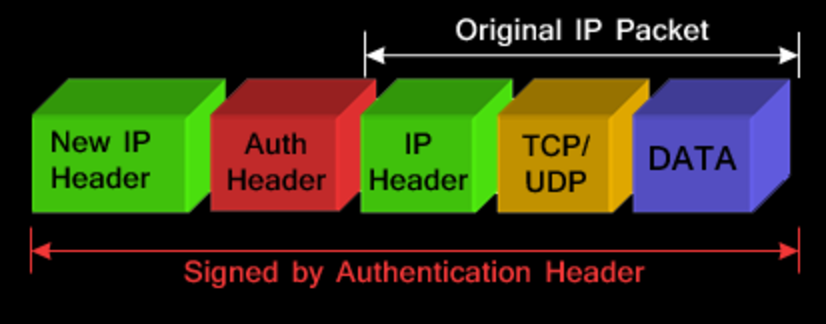
\includegraphics[scale=0.6]{ipsec-tunnel-ah.png}
\end{center}

\subsection{Combining SAs}
Multiple SAs may be combined into an SA bundle. An SA can only implement either AH or ESP, so in cases such as the following, one may combine more than one SA into a bundle:
\begin{itemize}
  \item To have both services and/or.
  \item Different flows in one communication path requires different services.
\end{itemize}
SAs can be combined into bundles in the following two ways:
\begin{itemize}
  \item \textbf{Transport Adjacency} - This refers to applying more than once security protocol to the same IP packet without invoking tunneling. This approach to combining AH and ESP allows for only one level of combination; further nesting yields no added benefit since the processing is performed at one IPsec instance: the ultimate destination.
  \item \textbf{Iterated tunneling} - This refers to the application of multiple layers of security protocols effected through IP tunneling. This approach allows for multiple levels of nesting, since each tunnel can originate or terminate at a different IPsec site along the path.
\end{itemize}

\subsection{Traffic Security Protocols}
Each of the IPSec traffic protocols defines a new set of headers to be added to IP datagrams. \textbf{Authentication Header (AH)} provides data origin authentication, data integrity and anti-replay but does not provide confidentiality protection.

\textbf{Encapsulating Security Payload (ESP)} provides:
\begin{itemize}
  \item Confidentiality protection (encryption)
  \item Partial traffic flow confidentiality
  \item data origin authentication, data integrity, anti-replay
\end{itemize}
ESP uses keyed-hash function, HMAC, for data integrity and authentication protection. It uses bulk encryption algorithms such as 3-key triple DES, AES, IDEA, CAST, Blowfish and RC5, for confidentiality protection.

\subsubsection{Authentication Header Format}
\begin{center}
  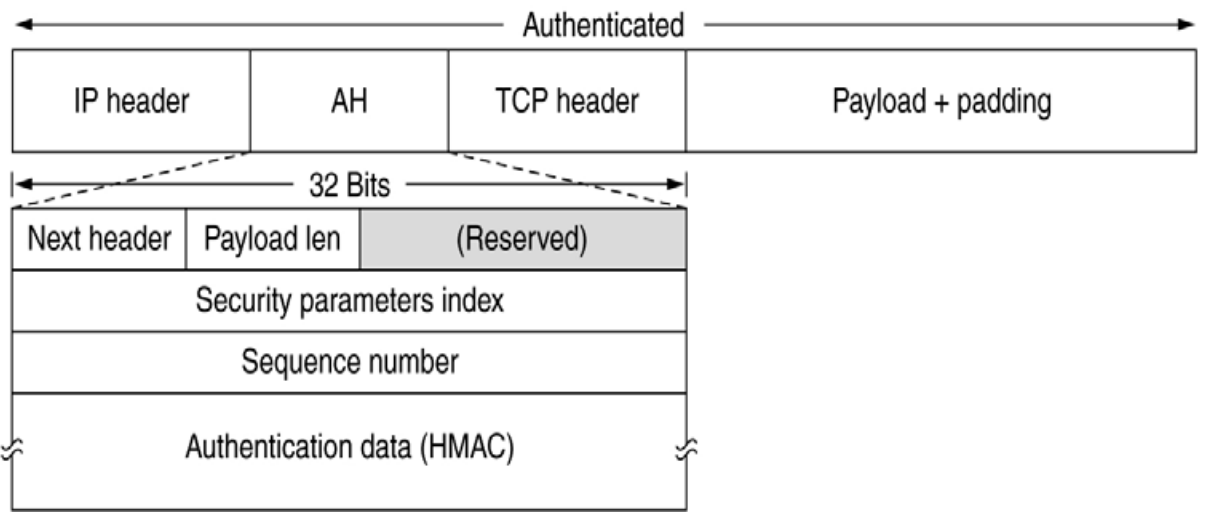
\includegraphics[scale=0.6]{ah-format.png}
\end{center}
\begin{itemize}
  \item NextHeader - specifies the type of header immediately following the Authentication Header.
  \item PayloadLength - The length of AH in 4-byte units.
  \item Reserves - not used now (set to 0)
  \item SPI - identifies a SA
  \item SequenceNumber - contains a monotonically increasing counter to protect against replay.
  \item AuthenticationData - contains the message authentication code (MAC) for this packet (typically 96 bits long)
\end{itemize}
The default MAC algorithm is HMAC built on a keyed one-way hash function. It is truncated to the first 96 bits and stored in the AH AuthenticationData field. The following rules are applied to IP Headers (transport mode) and new IP headers (tunnel mode) when computing the MAC:
\begin{itemize}
  \item Mutable IP header fields, e.g. TOS, flags, fragment offset, TTL and header checksum are zeroes prior to MAC calculation. All other immutable fields are included.
  \item The AH AuthenticationData field is zeroes. All other AH header fields are included.
  \item The entire upper-level protocol data are included.
\end{itemize}
Regarding integrity \& authentication. The following is done for an outbound packet (from the sender):
\begin{itemize}
  \item SA lookup
  \item Sequence number generation
  \item MAC calculation
\end{itemize}
And for the receiver:
\begin{itemize}
  \item Re-assemble (if IP packet has been fragmented)
  \item SA lookup
  \item Sequence number verification
  \item MAC verification
\end{itemize}
To prevent anti-replay the sequence number field is used. For a new SA, the sequence number is initialised as 1 for the first packet and increased by one for each outgoing packet up to $2^{32}-1$. If this limit is reached, then a new SA with a new key should be negotiated.

A window size, $W$, specifies the number of out-of-order packets that are tracked. The right edge of the window shows the highest sequence number, $N$, of the packet received so far. For packets with sequence numbers in the range from $N-W+1$ to $N$: if MAC is correct, then mark it, otherwise drop it. If a received packet is to the right of the window and is correctly authenticated, mark the packet and advance the window. If a received packet is to the left of the window, drop the packet:
\begin{center}
  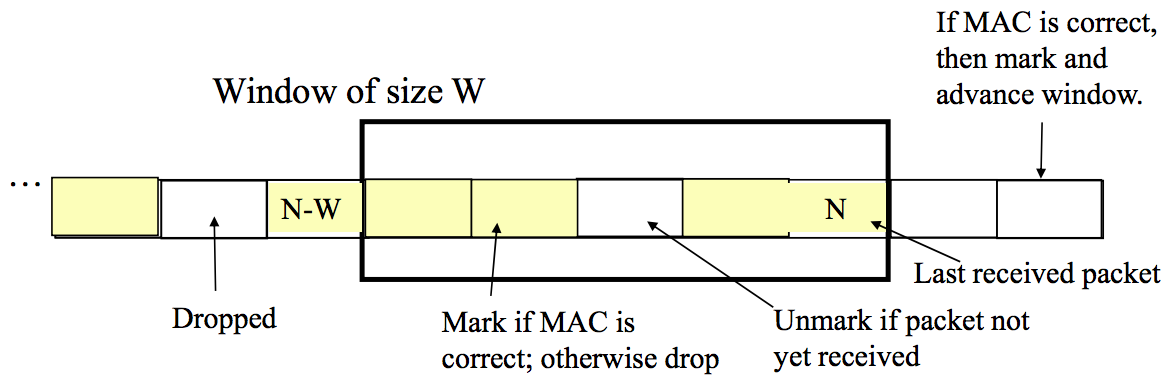
\includegraphics[scale=0.6]{ah-anti-replay.png}
\end{center}

\subsubsection{Encapsulating Security Payload Format}
\begin{center}
  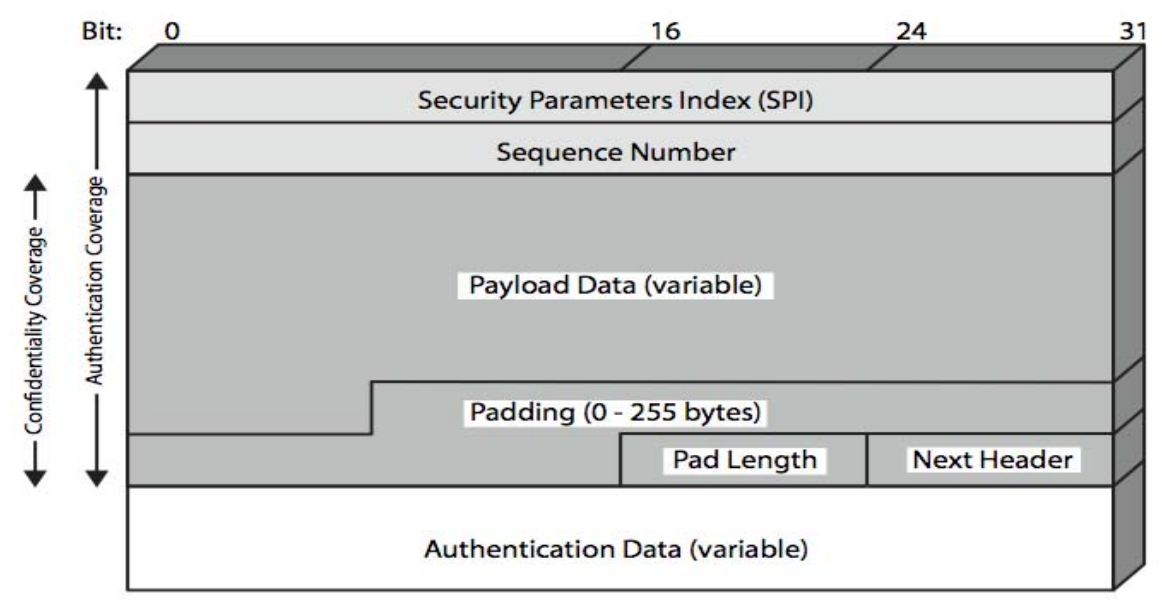
\includegraphics[scale=0.6]{esp-format.png}
\end{center}
Things here are similar to AH format. PayloadData is a transport level segment e.g. TCP segment (transport mode) or IP packet (tunnel mode) that is protected by encryption.

For outgoing packets first we have an SA lookup, then we have packet encryption:
\begin{itemize}
  \item Encapsulate relevant data into the ESP payload field.
  \item Add any necessary padding.
  \item Encrypts the result (PayloadData, Padding, PadLength, and NextHeader) using the key and the encryption algorithm  indicated by the SA.
\end{itemize}
Next we have sequence number generation and MAC calculation (if authentication is selected by the SA).

For inbound packets we perform re-assembly, SA lookup, sequence verification, MAC verification and packet decryption which involves:
\begin{itemize}
  \item Decrypt the relevant data.
  \item Process any padding as specifies in the encryption algorithm specification.
  \item Reconstructs the original IP datagram.
\end{itemize}

\subsubsection{Summary Table}
\begin{center}
  \begin{tabular}{|l|l|l|l|}
      \hline
      & AH & ESP & ESP with authentication \\ \hline
      Access control & \checkmark & \checkmark & \checkmark \\ \hline
      Connectionless integrity & \checkmark & & \checkmark \\ \hline
      Data origin authentication & \checkmark & & \checkmark \\ \hline
      Rejection of replayed attacks & \checkmark & & \checkmark \\ \hline
      Confidentiality & & \checkmark & \checkmark \\ \hline
      Limited traffic flow confidentiality & & \checkmark & \checkmark \\
      \hline
  \end{tabular}
\end{center}
\end{document}
